\chapter{Preliminary Work}\label{C:preliminary}

This chapter exhibits the two initial works for comprehensive quality-aware semantic web service composition approach, which combines a hybridization of various techniques for optimising the quality of semantic matchmaking and quality of service. In particular,  One direct representation and another indirect representation are proposed in two premilitary works using a PSO-based approach and a GP-based approach respectively. Apart from that, composition solutions are represented in a DAG or a tree-like representation,  respectively, in the two approaches. These two works are discussed in the following sections.

\section{Problem Formalisation}\label{problemDes}

We consider a \emph{semantic web service} (\emph{service}, for short) as a tuple $S =(I_{S}, O_{S}, $ $QoS_S)$ where $I_{S}$ is a set of service inputs that are consumed by $S$, $O_{S}$ is a set of service outputs that are produced by $S$, and $QoS_{S}=\{t_S, c_S, r_S, a_S\}$ is a set of non-functional attributes of $S$. The inputs in $I_{S}$ and outputs in $O_{S}$ are parameters modelled through concepts in a domain-specific ontology $\mathcal{O}$. The attributes $t_S, c_S, r_S, a_S$ refer to the response time, cost, reliability, and availability of service $S$, respectively. These four QoS attributes are most commonly used \cite{zeng2003quality}.

A \emph{service repository} $\mathcal{SR}$ is a finite collection of services supported by a common ontology $\mathcal{O}$. A \emph{service request} (also called \emph{composition task}) over $\mathcal{SR}$ is a tuple $T=(I_{T}, O_{T})$ where $I_{T}$ is a set of task inputs, and $O_{T}$ is a set of task outputs. The inputs in $I_{T}$ and outputs in $O_{T}$ are parameters described by concepts in the ontology $\mathcal{O}$.

%A service composition is commonly represented as a \emph{directed acyclic graph} (DAG). Its nodes correspond to the services in the composition. 
\emph{Matchmaking types} are often used to describe the level of a match between outputs and inputs \cite{paolucci2002semantic}: For concepts $a, b$ in $\mathcal{O}$ the \emph{matchmaking} returns $exact$ if $a$ and $b$ are equivalent ($a \equiv b$), $plugin$ if $a$ is a sub-concept of $b$ ($a \sqsubseteq b$), $subsume$ if $a$ is a super-concept of $b$ ($a \sqsupseteq b$), and $fail$ if none of previous matchmaking types is returned. In this paper we are only interested in robust compositions where only $exact$ and $plugin$ matches are considered, see \cite{lecue2009optimizing}. As argued in \cite{lecue2009optimizing} $plugin$ matches are less preferable than $exact$ matches due to the overheads associated with data processing. We suggest to consider the semantic similarity of concepts when comparing different $plugin$ matches.

\emph{Robust causal link} \cite{lecue2008optimizing} is a link between two matched services $S$ and $S'$, noted as $S \rightarrow S'$, if an output $a$ ($a \in {O_S}$) of $S$ serves as the input $b$ ($b \in {O_{S'}}$) of $S'$ satisfying either $a \equiv b$ or $a \sqsubseteq b$.  For concepts $a, b$ in $\mathcal{O}$ the \emph{semantic similarity} $sim(a, b)$ is calculated based on the edge counting method in a taxonomy like WorldNet or Ontology \cite{shet2012new}. This method has the advantages of simple calculation and good performance \cite{shet2012new}. Therefore, the \emph{matchmaking type} and \emph{semantic similarity} of a robust causal link can be defined as follow:
\begin{align}
\label{eq_link}
type_{link} = 
\begin{cases}
	1 & \text{ if $a\equiv b$ ($exact$ match)}\\
	p & \text{ if $a \sqsubseteq b$ ($plugin$ match)}
\end{cases}
,&&
sim_{link} = sim(a,b) = \frac{2N_c}{N_{a}+N_{b}}
\end{align}

\noindent with a suitable parameter $p, 0<p< 1$, and with $N_a$, $N_b$ and $N_c$, which measure the distances from concept $a$, concept $b$, and the closest common ancestor $c$ of $a$ and $b$ to the top concept of the ontology $\mathcal{O}$, respectively. However, if more than one pair of matched output and input exist from service $S$ to service $S'$, $type_{link}$ and $sim_{link}$ will take on their average values.

The \emph{semantic matchmaking quality} of the service composition can be obtained by aggregating over all robust causal links as follow:
\begin{align}
MT {=} \prod_{j=1}^{m} type_ {link_{j}}
,&&
SIM {=} \frac{1}{m}\sum_{j=1}^m sim_ {link_{j}}  
\end{align}

We consider two special atomic services $Start = (\emptyset, I_T, \emptyset )$ and $End  = (O_T, \emptyset, \emptyset)$ to account for the input and output requirements given by the composition task $T$, and add them to $\mathcal{SR}$. 

Given a service request $T=(I_T,O_T)$, we represent a service composition solution for $T$ with services $S_1,\ldots,S_n$  by a weighted DAG, $\gra=(V,E)$ with node set $V=\{Start, S_1, S_2, $ $\ldots, S_n, End\}$ and edge set $E = \{link_{1}, link_{2},... link_{m} \}$. Each edge $link$ is a \emph{robust causal link}.


We also use formal expressions as in \cite{ma2012formal} to represent service compositions. We use the constructors $\bullet$, $\parallel$, $+$ and $\ast$ to denote sequential composition, parallel composition, choice, and iteration, respectively. The set of \emph{composite service expressions} is the smallest collection $\mathcal{SC}$ that contains all atomic services and that is closed under sequential composition, parallel composition, choice, and iteration. That is, whenever $\cse_0,\cse_1,\ldots,\cse_d$ are in $\mathcal{SC}$ then $\bullet(\cse_1,\ldots,\cse_d)$, $\parallel(\cse_1,\ldots,\cse_d)$, $+(\cse_1,\ldots,\cse_d)$, and $\ast \cse_0$ are in $\mathcal{SC}$, too. Let $\cse$ be a composite service expression. If $\cse$ denotes an atomic service $S$ then its QoS is given by $QoS_S$.  Otherwise the QoS for $\cse$ can be obtained inductively as summarized in Table~\ref{tbl:QoS_Aggre}. Herein, $p_1,\ldots,p_d$ with $\sum\limits^d_{k=1}p_k=1$ denote the probabilities of the different options of the choice $+$, while $\ell$ denotes the average number of iterations.

\begin{table}[htb]
\centering
\caption{QoS calculation for a composite service expression $\cse$}
\begin{tabular}{l|l|l|l|l}
\hline
 $\cse=$       &$r_\cse=$                              &$a_\cse=$                              &$c_\cse=$                            &$t_\cse=$ \\ \hline
 $\bullet(\cse_1,\ldots,\cse_d)$      &$\prod\limits^d_{k=1}r_{\cse_k}$    &$\prod\limits^d_{k=1}a_{\cse_k}$    &$\sum\limits^d_{k=1}c_{\cse_k}$   &$\sum\limits^d_{k=1}t_{\cse_k}$  \\ \hline
 $\parallel(\cse_1,\ldots,\cse_d)$  &$\prod\limits^d_{k=1}r_{\cse_k}$    &$\prod\limits^d_{k=1}a_{\cse_k}$    &$\sum\limits^d_{k=1}c_{\cse_k}$   &$MAX \{ t_{\cse_k} | k \in \{ 1,...,d \} \}$\\ \hline
 $+(\cse_1,\ldots,\cse_d)$     &$\prod\limits^d_{k=1}p_k\cdot r_{\cse_k}$    &$\prod\limits^d_{k=1}p_k\cdot a_{\cse_k}$    &$\sum\limits^d_{k=1}p_k\cdot c_{\cse_k}$   &$\sum\limits^d_{k=1}p_k\cdot t_{\cse_k}$  \\ \hline
 $\ast \cse_0$         &${r_{\cse_0}}^\ell$  &${a_{\cse_0}}^\ell$  &$\ell\cdot c_{\cse_0}$ &$\ell\cdot t_{\cse_0}$ \\ \hline
\end{tabular}
\label{tbl:QoS_Aggre}
\end{table}

When multiple quality criteria are involved in decision making, the fitness of a solution can be defined as a weighted sum of all individual criteria using Eq. (\ref{eq_fitness}), assuming the preference of each quality criterion is provided by users.
\begin{equation}
\label{eq_fitness}
Fitness = w_1 \hat{MT} + w_2 \hat{SIM} + w_3 \hat{A} + w_4 \hat{R} + w_5(1 - \hat{T}) + w_6(1 - \hat{C})
\end{equation}
\noindent with $\sum_{k=1}^{6} w_k= 1$. We call this objective function the \emph{comprehensive quality model} for service composition.
The weights can be adjusted according to users' preferences. $\hat{MT}$, $\hat{SIM}$, $\hat{A}$, $\hat{R}$, $\hat{T}$, and $\hat{C}$ are normalised values calculated within the range from 0 to 1 using Eq. (\ref{eq_normal}). To simplify the presentation we also use the notation $(Q_1,Q_2,Q_3,Q_4,Q_5,Q_6) $ $= (MT,SIM,A,R,T,C)$. $Q_1$ and $Q_2$ have minimum value 0 and maximum value 1. The minimum and maximum value of $Q_3$, $Q_4$, $Q_5$, and $Q_6$ are calculated across all task-related candidates in the service repository $\mathcal{SR}$ using the greedy search in \cite{ma2015hybrid,da2016genetic}.

\begin{equation}
\label{eq_normal}
\hat{Q_k} = 
\begin{cases}
	\frac{Q_k - Q_{k, min}}{Q_{k, max} - Q_{k, min}} & \text{ if $k=1,\ldots,4$ and }Q_{k, max} - Q_{k, min} \neq 0,\\
	\frac{Q_{k,max} - Q_k}{Q_{k, max} - Q_{k, min}} & \text{ if $k=5,6$ and }Q_{k, max} - Q_{k, min} \neq 0,\\
	1 & \text{ otherwise}.
\end{cases}
\end{equation}

\noindent To find best possible solution for a given composition task $T$, our goal is to maximise the objective function in Eq. (\ref{eq_fitness}).


\section{PSO-based Approach to Comprehensive Quality-Aware Automated Semantic Web Service Composition}\label{qswsc_approach}
\subsection{An Overview of our PSO-based Approach}\label{PSO_based_approach}
As PSO has shown promise in solving combinatorial optimisation problems, we propose a PSO-based approach to comprehensive quality-aware automated semantic web service composition. Fig. \ref{overview} shows an overview of our approach consisting of four steps: 
\begin{figure}[h]
\centering
\fbox{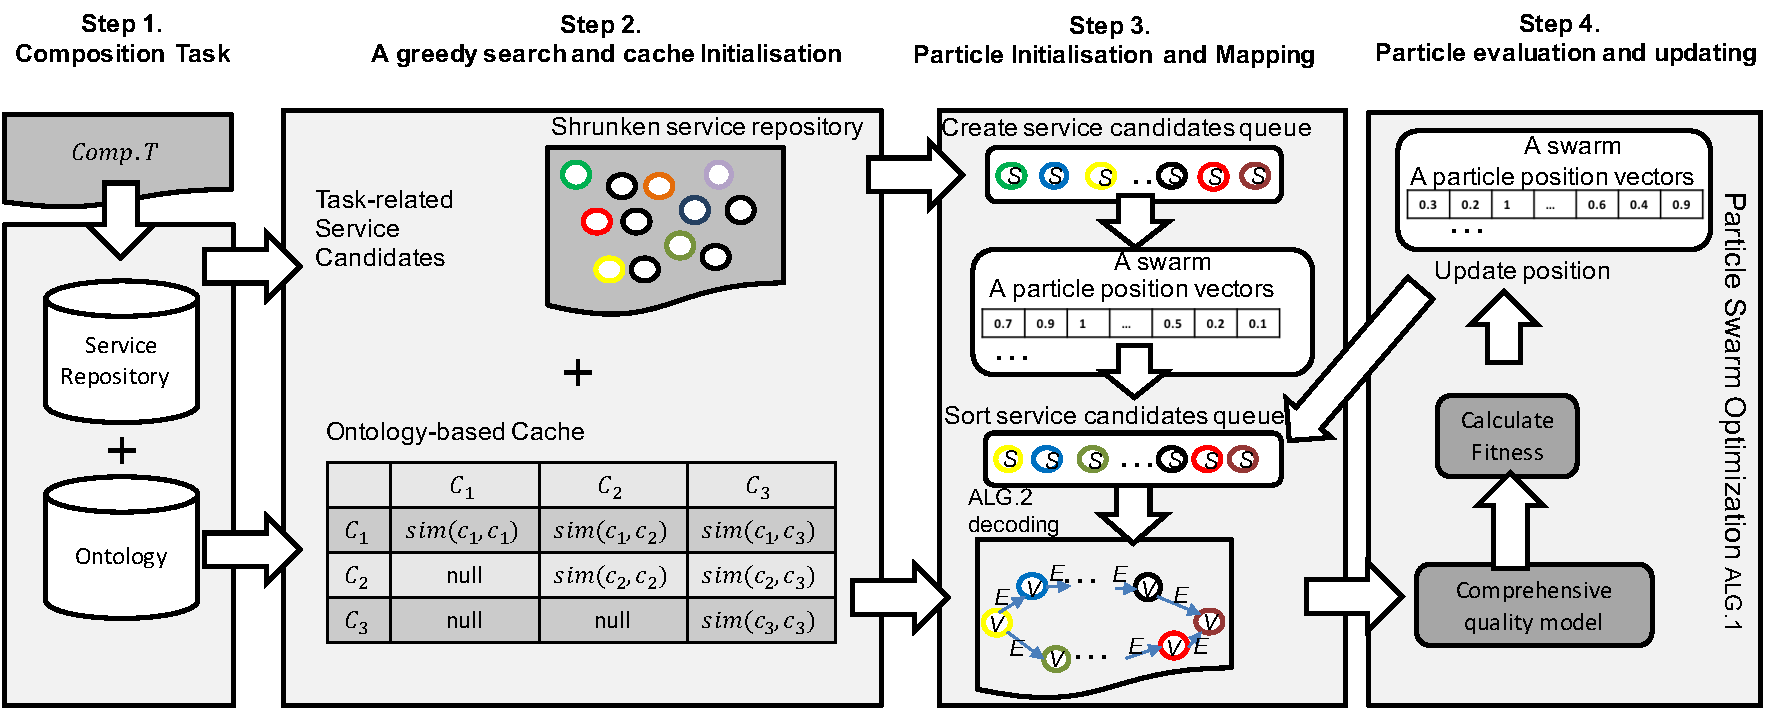
\includegraphics[scale=.5]{overview.pdf}}
 \caption{An overview of our PSO-based approach to comprehensive quality-aware automated semantic web service composition.}
 \label{overview}
\end{figure}

Step 1: The composition process is triggered by a composition task, which is clearly defined in Section \ref{problemDes}. 

Step 2: The composition task is used to discover all task-related service candidates using a greedy search algorithm adopted from \cite{ma2015hybrid}, which contributes to a shrunken service repository. This greedy search algorithm keeps adding outputs of the invoked services as available outputs (initialised with $I_{T}$) , and these available outputs are used to discover task-related services from a service repository and updated with the outputs of these discovered services. This operation is repeated until no service is satisfied by the available outputs. During the greedy search, an ontology-based cache ($cache$) is initialised, which stores the concept similarities of matched inputs and outputs of task-related candidates. This $cache$ is also used to discover services by checking whether $null$ is returned by given two output-related and input-related concepts.

Step 3 and Step 4: These two steps follow the standard PSO steps \cite{shi2001particle} except for some differences in particles mapping and decoding processes. In particular, these two differences are related to sorting a created service queue using service-to-index mapping for a particle' position vectors and evaluating the fitness of a particle after decoding this service queue into a $\gra$ respectively. Those differences are further addressed in Algorithms \ref{novelSteps} and \ref{graph_building} in Section \ref{PSO-based_algomargin}.
\subsection{The Algorithms for our PSO-based Approach}\label{PSO-based_algomargin}
The overall algorithm investigated here is made up of a PSO-based web service composition technique (Algorithm \ref{novelSteps}) and a $\gra$ creating technique from a service queue (Algorithm \ref{graph_building}). In Algorithm \ref{novelSteps}, the  steps $4$, $5$, $6$ and $7$ are different from those of standard PSO: In step 4, the size of task-related service candidates generated by a greedy search determines the size of each particle's position. Each service candidate in a created service candidates queue is mapped to an index of a particle’s position vectors, where each vector has a weight value between 0.0 and 1.0. In step 5, service candidates in the queue are sorted according to their corresponding weight values in descending order. In step 6, this sorted queue is used as one of the inputs of the forward decoding Algorithm \ref{graph_building} to create a $\gra$. In step 7, the fitness value of the created $\gra$ is the fitness value of the particle calculated by the comprehensive model discussed in Section \ref{problemDes}.
\begin{algorithm}
 %\LinesNumbered
 \SetKwInOut{Input}{Input}\SetKwInOut{Output}{Output}
 \SetKwFunction{generateWeightedGraph}{generateWeightedGraph}
 \SetKwProg{Procedure}{Procedure}{}{}
 \SetNlSty{}{}{:}
 Randomly initialise each particle in the swarm\;
  \While {max. iterations not met}{
     \ForEach{particle in the swarm}{
     Create a service candidates queue and map service candidates to a particle's position vectors\;
     Sort the service queue by position vectors' weights\;
     Use Algorithm \ref{graph_building} to create a $\gra$ from the service queue\;
     Calculate the $\gra$ fitness value\;
     
      \eIf{fitness value better than pBest}{    
        Assign current fitness as new \emph{pBest}\;
       }{
        Keep previous \emph{pBest}\;
       }	
     }
    Assign best particle's \emph{pBest} value to \emph{gBest}, if better than \emph{gBest}\;
 	Calculate the velocity of each particle\;
  	Update the position of each particle\;
  }
\caption{Steps of PSO-based service composition technique \cite{da2016particle}.}
\label{novelSteps}
\end{algorithm} 

Algorithm  \ref{graph_building} is a forward graph building algorithm extended from \cite{blum1997fast}. This algorithm takes one input, a sorted service queue from step 5 of Algorithm \ref{novelSteps}. Note that different service queues may lead to different $\gra$s. In addition. $I_{T}$, $O_{T}$ and $cache$ are also taken as the inputs. Firstly, $Start$ and $End$ are added to $V$ of $\gra$ as an initialisation, and $OutputSet$ is also created with $I_{T}$. The following steps are repeated until $O_{T}$ can be satisfied by $Outputset$ or the service queue is $null$. If all the inputs $I_{S}$ of the first popped  $S$ from $queue$ can be satisfied by provided outputs from $OutputSet$, this $S$ is added to $V$ and its outputs are added to $OutputSet$, and $S$ is removed from $queue$. Otherwise, the second popped  $S$ from $queue$ is considered for these operations. Meanwhile, $link$ is created with $type_{link}$ and $sim_{link}$ if $S$ is added, and calculated using information provided from $cache$. This forward graph building technique could lead to more services and edges connected to the $\gra$, these redundancies should be removed before $\gra$ is returned.

\begin{algorithm}
 \SetKwInOut{Input}{Input}\SetKwInOut{Output}{Output}
 \SetKwFunction{createWeightedDAG}{createWeightedDAG}
 \SetKwProg{Procedure}{Procedure}{}{}
 %\LinesNumbered
 \SetNlSty{}{}{:}
 % \Procedure{}{
 \Input{ $I_T$, $O_T$, $queue$, $cache$}
 \Output{$\gra$}
 $\gra = (V, E)$\;
 $V \leftarrow$ \{$Start$, $End$ \}\;
 $OutputSet \leftarrow$ \{$I_{T}$\}\;
  \While { $O_{T}$ not satisfied by $OutputSet$}{
     \ForEach{$S$ in $queue$}{
      \uIf{$I_{S}$ satisfied by $OutputSet$}{  
        insert $S$ into $V$\;  
        adjoin $O_{S}$ to $OutputSet$\;
        $queue$.remove $S$\;   
        $link \leftarrow$ calculate $type_{link}$, $sim_{link}$ using $cache$\;
        insert $link$ into $E$\;
       }	
     }
  }
 remove $dangling$ $nodes$ and $edges$ from $\gra$\; 
 \KwRet $\gra$\;
 %}
 \caption{Create a $\gra$ from a sorted service queue.}
\label{graph_building}
\end{algorithm} 

\section{Experiment Study for PSO-based Approach}\label{experiment_design}
In this section, we employ a quantitative evaluation approach with a benchmark dataset used in \cite{ma2015hybrid,da2016genetic}, which is an augmented version of Web Service Challenge 2009 (WSC09) including QoS attributes. Two objectives of this evaluation are to: $(1)$ evaluate the effectiveness of our PSO-based approach, see comparison test in Section \ref{comparisonTestWithGP}. $(2)$ evaluate the effectiveness of our proposed comprehensive quality model to achieve a desirable balance on semantic matchmaking quality and QoS, see comparison test in Section \ref{comparisonTest}.

The parameters for the PSO are chosen from the settings from \cite{shi2001particle}, In particular, PSO population size is 30 with 100 generations. We run 30 times independently for each dataset. We configure the weights of fitness function to properly balance semantic matchmaking quality and QoS. Therefore, $w_{1}$ and $w_{2}$ are set equally to 0.25, and $w_{3}$, $w_{4}$, $w_{5}$, $w_{6}$ are all set to 0.125. The $p$ of $type_{link}$ is set to 0.75 ($plugin$ match) according to \cite{lecue2009optimizing}. In general, weight settings and parameter $p$ are decided according to users' preferences.

\subsection{GP-based vs. PSO-based approach}\label{comparisonTestWithGP}
To evaluate the effectiveness of our proposed PSO-based approach, we compare our PSO-based method with one recent GP-based approach \cite{ma2015hybrid} using our proposed comprehensive quality model. We extend this GP-based approach by measuring the semantic matchmaking quality between parent nodes and children nodes. To make a fair comparison, we use the same number of evaluations (3000 times) for these two approach. We set the parameters of that GP-based approach as 30 individuals and 100 generations, which is considered to be proper settings referring to \cite{da2015gp}.

The first column of Table \ref{meanFitness} shows five tasks from WSC09. The second and third column of Table \ref{meanFitness} show the original service repository size and the shrunk service repository size after the greedy search respectively regarding the five tasks. This greedy search helps reducing the original repository size significantly, which contributes to a reduced searching space. The fourth and fifth column of Table \ref{meanFitness} show the mean fitness values of 30 independent runs accomplished by two methods. We employ independent-samples T tests to test the significant differences in mean fitness value. The results show that the PSO-based approach outperforms the existing GP-based approach in most cases except Task 3. Note that all $p$-values are consistently smaller than 0.01. Using our PSO-based approach, small changes to sorted queues (particles in PSO) could lead to big changes to the composition solutions. This enables the PSO-based approach to escape from local optima more easily than the GP-based approach. 
%the PSO-based approach performs significantly better than the GP-based approach in finding optimal solutions. It may be that the GP-based approach is stuck in local optima in a very large search space due to its evolutionary operators. On the other hand, the decoding process used by the PSO-based approach allows for small changes that more effectively prevent this from happening.
\begin{table}[]
\centering
\caption{Mean fitness values for comparing GP-based approach}
\label{meanFitness}
\begin{tabular}{c|c|c|l|l}
\hline
\multicolumn{1}{c|}{WSC09} &Original $\mathcal{SR}$  &Shrunken $\mathcal{SR}$   &PSO-based approach & GP-based approach  \\ \hline
Task 1                     &572            &80    &0.5592 $\pm$ 0.0128  $\uparrow$  &0.5207 $\pm$ 0.0208           \\ \hline
Task 2                     &4129           &140   &0.4701 $\pm$ 0.0011  $\uparrow$  &0.4597 $\pm$ 0.0029          \\ \hline
Task 3                     &8138           &153   &0.5504 $\pm$ 0.0128              &0.5679 $\pm$ 0.0234 $\uparrow$   \\ \hline
Task 4                     &8301           &330   &0.4690 $\pm$ 0.0017  $\uparrow$  &0.4317 $\pm$ 0.0097            \\ \hline
Task 5                     &15211          &237   &0.4694 $\pm$ 0.0008  $\uparrow$  &0.2452 $\pm$ 0.0369            \\ \hline
\end{tabular}
\end{table}

\subsection{Comprehensive Quality Model vs. QoS Model}\label{comparisonTest}

Recently, a QoS Model, $Fitness = w_1 \hat{A} + w_2 \hat{R} + w_3(1 - \hat{T}) + w_4(1 - \hat{C})$, where $\sum_{i=1}^{4} w_i = 1$, is widely used for QoS-aware web service composition \cite{ma2015hybrid,da2016particle,da2015graphevol}. To show the effectiveness of our proposed comprehensive quality model, we compare the best solutions found by this QoS model and our comprehensive model using our PSO-based approach. We record and compare the mean values of both $SM$ ($SM = 0.5 \hat{MT} + 0.5 \hat{SIM}$) and $QoS$($QoS = 0.25 \hat{A} + 0.25 \hat{R} + 0.25(1 - \hat{T}) + 0.25(1 - \hat{C})$) of best solutions over 30 independent runs. To make the comparison informative, all these recorded values have been normalised from 0 to 1, and compared using independent-samples T tests, see Table \ref{decisionTable}. Note that p-values are consistently smaller than 0.001 in the results indicating significant differences in performance. 

In Table \ref{decisionTable}, the mean values of $QoS$ using QoS model are significantly higher than those using comprehensive quality model for Tasks 2, 3, 4 and 5. However, the mean value of $SM$ using the comprehensive quality model are significantly higher than those using the QoS model, while a slight trade-off in $QoS$ are observed in all tasks. In addition, our comprehensive model achieves a consistently higher comprehensive quality in terms of a combination of $SM$ and $QoS$, which is significantly better in Tasks 1, 2, 3 and 4. 
\begin{table}[]
\footnotesize
\centering
\caption{Mean values of $SM$, $QoS$ and sum of $SM$ and $QoS$ for QoS model and comprehensive quality model using PSO-based approach}
\label{decisionTable}
\begin{tabular}{c|c|l|l}
\hline
\multicolumn{2}{c|}{WSC09}              & \shortstack{QoS \\ Model}         &\shortstack{Comprehensive Quality \\ Model} \\ \hline
\multirow{3}{*}{Task1}  &$SM$      &0.5373 $\pm$ 0.0267               &0.5580 $\pm$ 0.0094 $\uparrow$ \\ \cline{2-4}
                        &$QoS$     &0.5574 $\pm$ 0.0156               &0.5604 $\pm$ 0.0164            \\ \cline{2-4}
                        &$SM+QoS$  &1.0947 $\pm$ 0.0423               &1.1184 $\pm$ 0.0258 $\uparrow$ \\ \hline
\multirow{3}{*}{Task2}  &$SM$      &0.4549 $\pm$ 0.0033               &0.4630 $\pm$ 0.0042 $\uparrow$ \\ \cline{2-4} 
                        &$QoS$     &0.4800 $\pm$ 0.0012 $\uparrow$    &0.4772 $\pm$ 0.0025            \\ \cline{2-4}
                        &$SM+QoS$  &0.9349 $\pm$ 0.0045               &0.9402 $\pm$ 0.0067 $\uparrow$           \\ \hline
\multirow{3}{*}{Task3}  &$SM$      &0.5538 $\pm$ 0.0082               &0.6093 $\pm$ 0.0054 $\uparrow$ \\ \cline{2-4} 
                        &$QoS$     &0.4940 $\pm$ 0.0013 $\uparrow$    &0.4913 $\pm$ 0.0009            \\ \cline{2-4}
                        &$SM+QoS$  &1.0478 $\pm$ 0.0095               &1.1006 $\pm$ 0.0063 $\uparrow$           \\ \hline
\multirow{3}{*}{Task4}  &$SM$      &0.4398 $\pm$ 0.0037               &0.4604 $\pm$ 0.0000 $\uparrow$ \\ \cline{2-4} 
                        &$QoS$     &0.4845 $\pm$ 0.0010 $\uparrow$    &0.4734 $\pm$ 0.0044            \\ \cline{2-4}
                        &$SM+QoS$  &0.9243 $\pm$ 0.0047               &0.9338 $\pm$ 0.0044 $\uparrow$           \\ \hline
\multirow{3}{*}{Task5}  &$SM$      &0.4580 $\pm$ 0.0065               &0.4639 $\pm$ 0.0013 $\uparrow$ \\ \cline{2-4} 
                        &$QoS$     &0.4764 $\pm$ 0.0005 $\uparrow$    &0.4750 $\pm$ 0.0007            \\ \cline{2-4}
                        &$SM+QoS$  &0.9344 $\pm$ 0.0070               &0.9389 $\pm$ 0.0020           \\ \hline
\end{tabular}
\end{table}
\subsection{Further Discussion}\label{discuss1}
To analyse the effectiveness of achieving a good comprehensive quality at the expense of slightly reduced QoS, we demonstrate two best solutions produced using Task 3 as an example. Fig. \ref{comparisontest} $(1)$ and $(2)$ show two weighted DAGs, $\gra_1$ and $\gra_2$, which have been obtained as the best service compositions solutions based on the QoS model and on the comprehensive quality model, respectively. Both $\gra$s have exactly the same service workflow structure, but some service vertices and edges denoted in red are different. To better understand these differences, we list the overall semantic matchmaking quality $SM$,  overall $QoS$ and semantic matchmaking quality $sm_{link_n}$ associated to these different edges in $\gra_1$ and $\gra_2$. (Note: $sm_{link_n} = 0.5type_{link_n} + 0.5 sim_{e_n}$), where $\Delta Q$ reveals the gain (positive $\Delta Q$) or a loss (negative $\Delta Q$) of the listed qualities for our comprehensive quality model. Therefore, we achieve a comprehensive quality gain (+0.1433), a result of a gain in semantic matchmaking quality (+0.1467) and a loss in $QoS$ (-0.0034). To understand the improvement of semantic matchmaking quality from these numbers, we pick up $link_4$ that is associated with the smallest $\Delta Q$. The $link_4$ of $\gra_1$ and $\gra_2$ has two different source nodes, $Ser1640238160$ and $Ser947554374$, and two the same $End$ nodes. $Ser1640238160$ and $Ser947554374$ are services with output parameters $Inst582785907$ and  $Inst795998200$ corresponds to two concepts $Con2037585750$ and $Con103314376$ respectively in the given ontology shown in Fig. \ref{comparisontest} $(4)$. As $Inst658772240$ is a required parameter of $End$, and related to concept $Con2113572083$, $Inst795998200$ is closer to the required output $Inst658772240$ than $Inst582785907$. Therefore,  $Ser947554374$ is selected with a better semantic matchmaking quality compared to $Ser1640238160$.
\begin{figure}[h]
\centering{
\fbox{
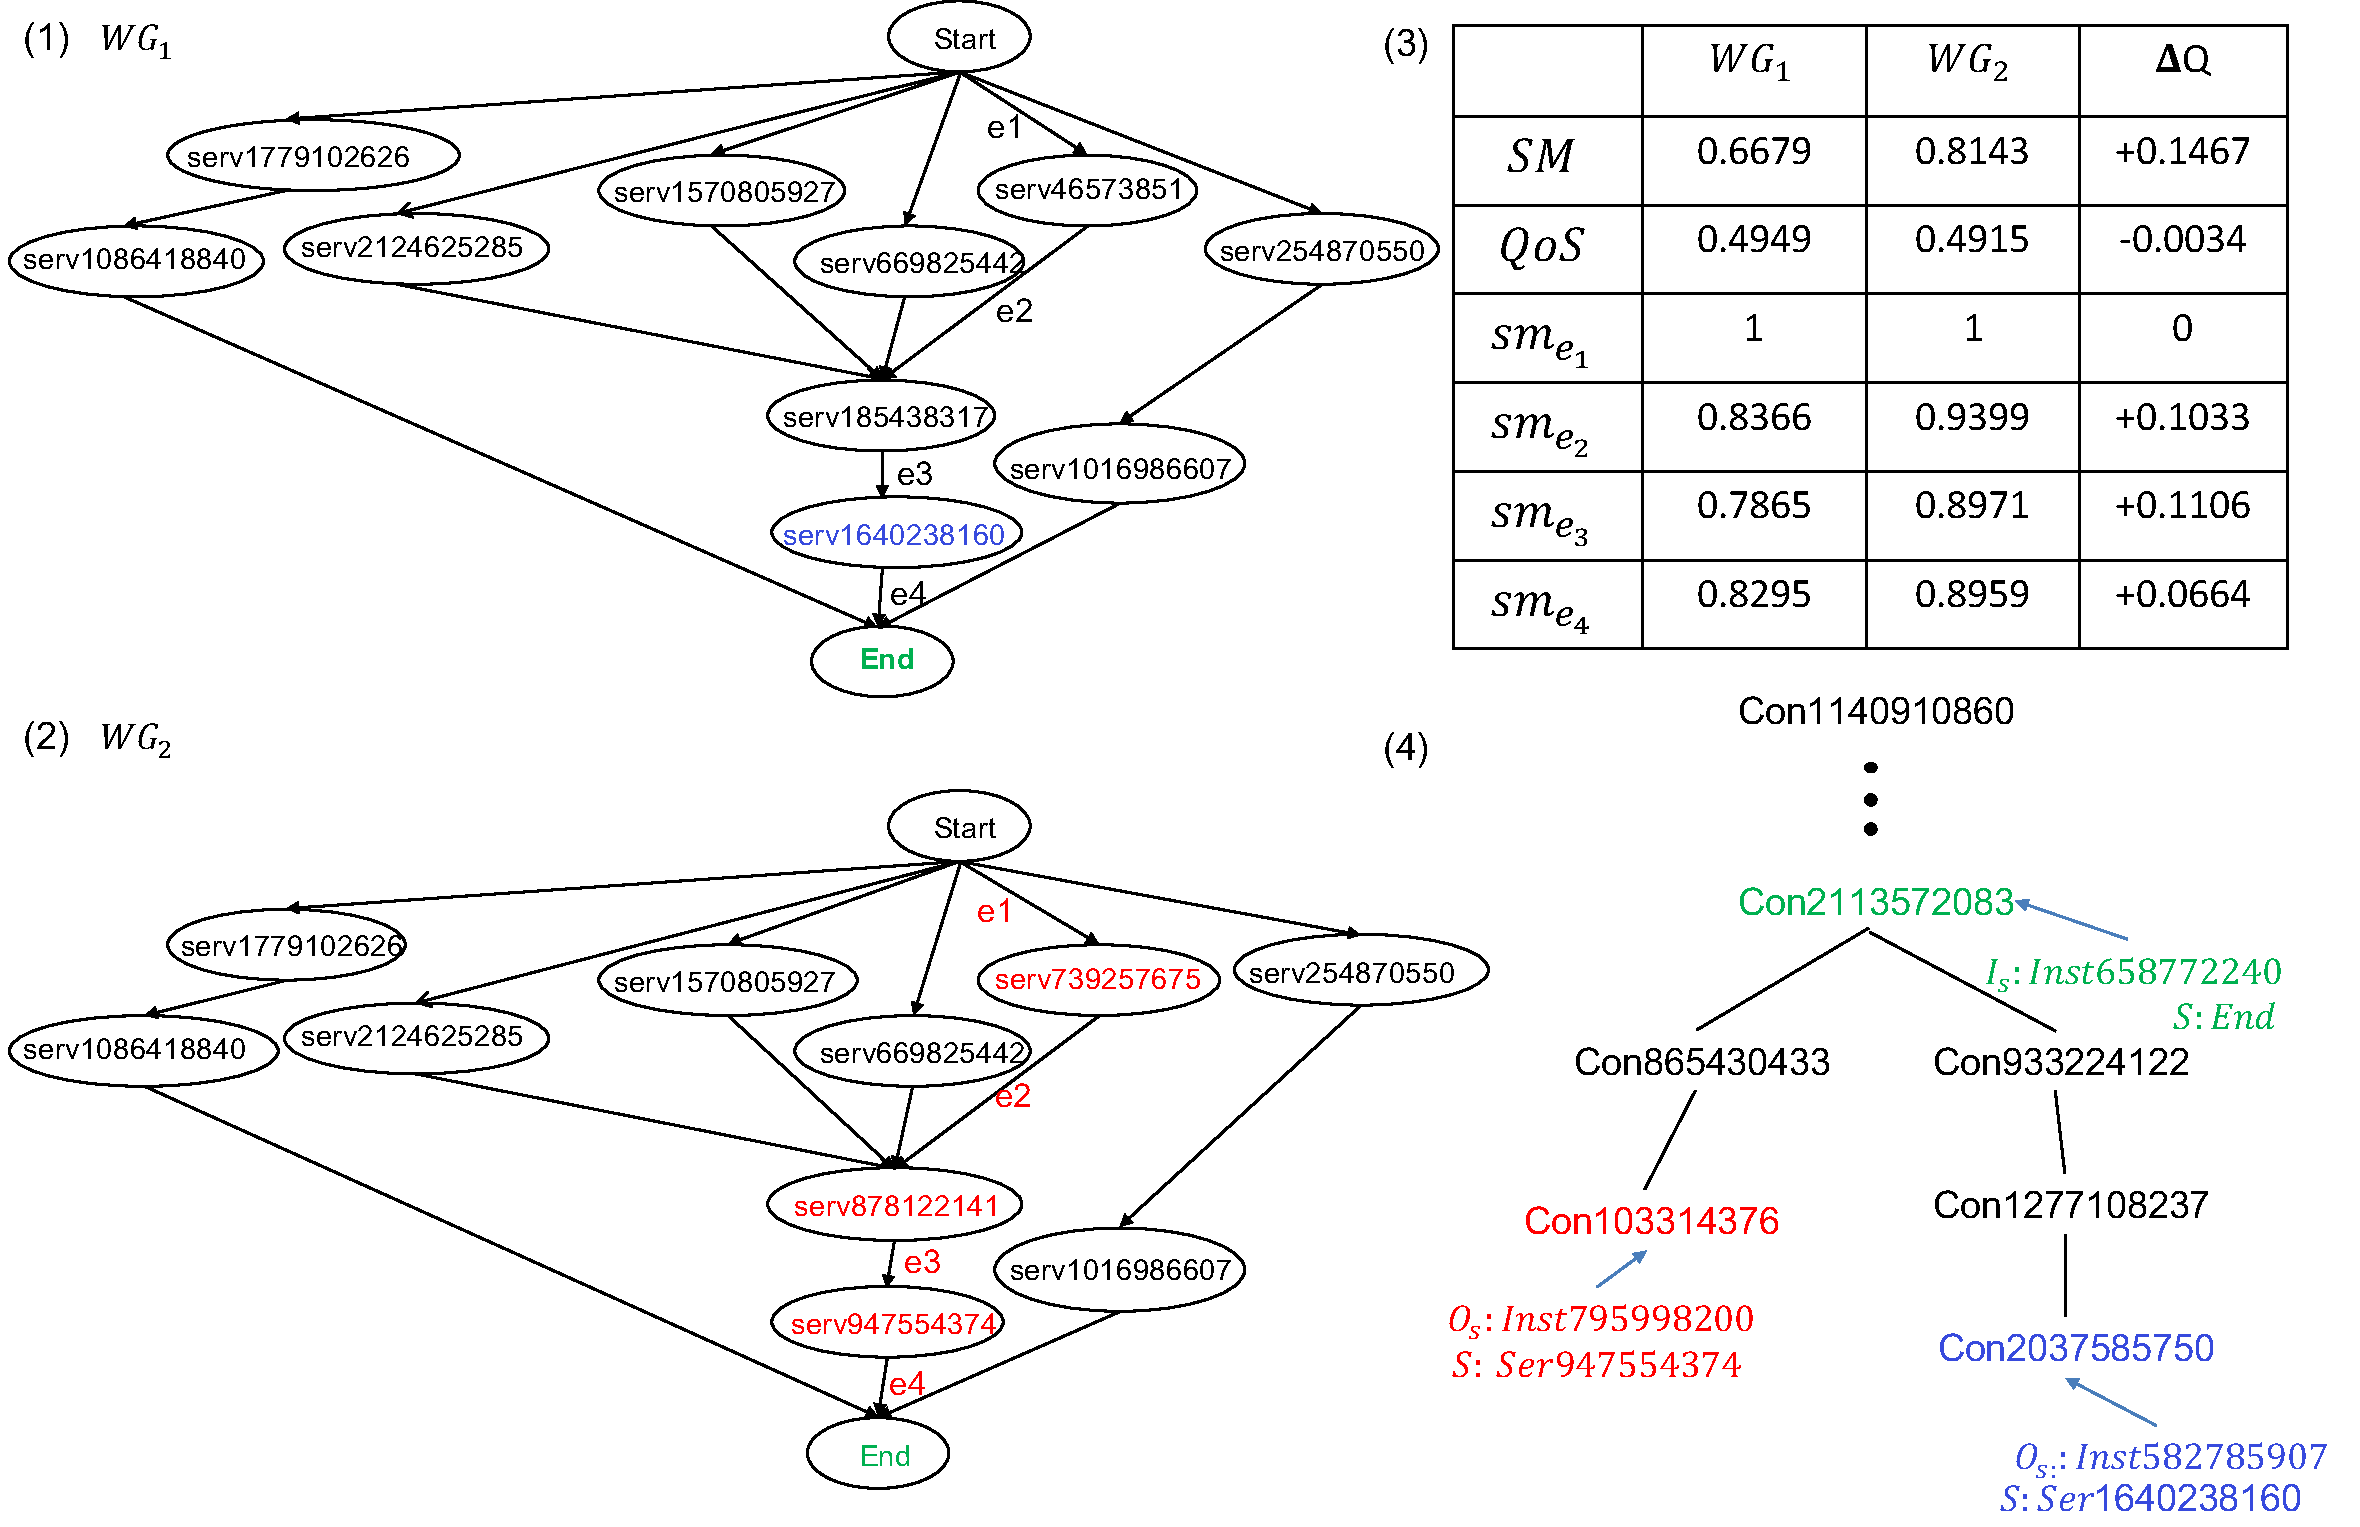
\includegraphics[scale=.29]{comparisontest.pdf}}}
 \caption{An example for the comparison of the best solutions obtained based on the QoS model and on the comprehensive quality model for Task 3.}
 \label{comparisontest}
\end{figure}

\section{Summary for our PSO-based Approach}\label{summary1}

In PSO-based approach, we propose an effective PSO-based approach to comprehensive quality-aware semantic web service composition, which also has shown promise in achieving a better comprehensive quality in terms of a combination of semantic matchmaking quality and QoS compared to existing works.
%=================================================================================================== GP Approach
\section{GP-based Approach to Comprehensive Quality-Aware Automated Semantic Web Service Composition}\label{GPApproach}

In this section, we first introduce the tree-like representation that will be used in our approach, and then discuss the differences to the most widely used tree-based representations for GP-based service composition in the literature \cite{gupta2015optimization,da2016genetic,yu2013adaptive}. Finally, we present our GP-based approach with newly designed genetic operation methods.
%========================================================================================= Representation
\subsection{A New Tree-like Representation for Web Service Composition}\label{representation} 

Let $\gra=(V,E)$ be a weighted DAG representation of a service composition. Let $S$ be a service in $\gra$, and let $S_1,\ldots,S_d$ be its successors in $\gra$. We define the composite service expression relative to $S$ as follows: 
\begin{equation}
\label{eq_s_expression}
    \cse_S=
    \begin{cases}
      \bullet(S,\parallel(\cse_{S_1},\ldots,\cse_{S_d})), & \text{if $d\ge 2$}, \\
      \bullet(S,\cse_{S_1}), & \text{if $d=1$}, \\
      S, & \text{if $d=0$},
    \end{cases}
\end{equation}
which can be evaluated inductively starting with $Start$ which has no incoming edges in $\gra$. The resulting expression $C_{Start}$ is a composite service expression that is equivalent to $\gra$.
%Note: This needs to be modified slightly if there can be more nodes without incoming edges (other than Start). 

\begin{example}
Consider the composition task $T=(\{a, b, e\},\{ i\})$. Fig.~\ref{fig:ExampleOfRepresentation} shows an example of a composition solution. It involves four atomic services $S_1=(\{a, b \}, \{c, d, j \}, QoS_{S_1})$, $S_2=(\{c \}, \{f, g \}, QoS_{S_2})$, $S_3=(\{d \}, \{h \}, QoS_{S_3})$, and $S_4=(\{f, g, h \}, \{ i \}, QoS_{S_4})$. The two special services $Start=(\emptyset,\{a,b,e\},\emptyset)$ and $End=(\{i\},\emptyset,\emptyset)$ are defined by the given composition task $T$. The corresponding service composition expression is:

\noindent $\cse_{Start}=\bullet(Start,\bullet( S_1,\parallel(\bullet(S_2,\bullet(S_4,End)),\bullet(S_3,\bullet(S_4,End))))).$
\end{example}

Formal expressions can be visualized by expressions trees. For a composite service expression $\cse$ let $\tree$ denote the corresponding expression tree. 
%Let $V_t$ and $V_f$ denote the leaf nodes (also called \emph{terminal nodes}) and the internal nodes (also called \emph{functional nodes}) of $\tree$. 
Every leaf node in $\tree$ is labelled by the corresponding atomic service, while every internal node in $\tree$ is labelled by the corresponding composition constructor. For the sake of brevity we only consider $\bullet$ and $\parallel$ here, but our approach can easily be extended to $+$ and $\ast$, too. If a subtree of $\tree$ (except for $End$) has an isomorphic copy in $\tree$ then we remove it, label its root with a special symbol $q$, and insert an edge to the root of the copy. As a result we obtain a tree-like representation of a service composition. An example is shown in Fig.~\ref{fig:ExampleOfRepresentation}.

\begin{figure}[h!tb]
\centering
%\fbox{\includegraphics[scale=.30]{synthesisRules.pdf}}
\fbox{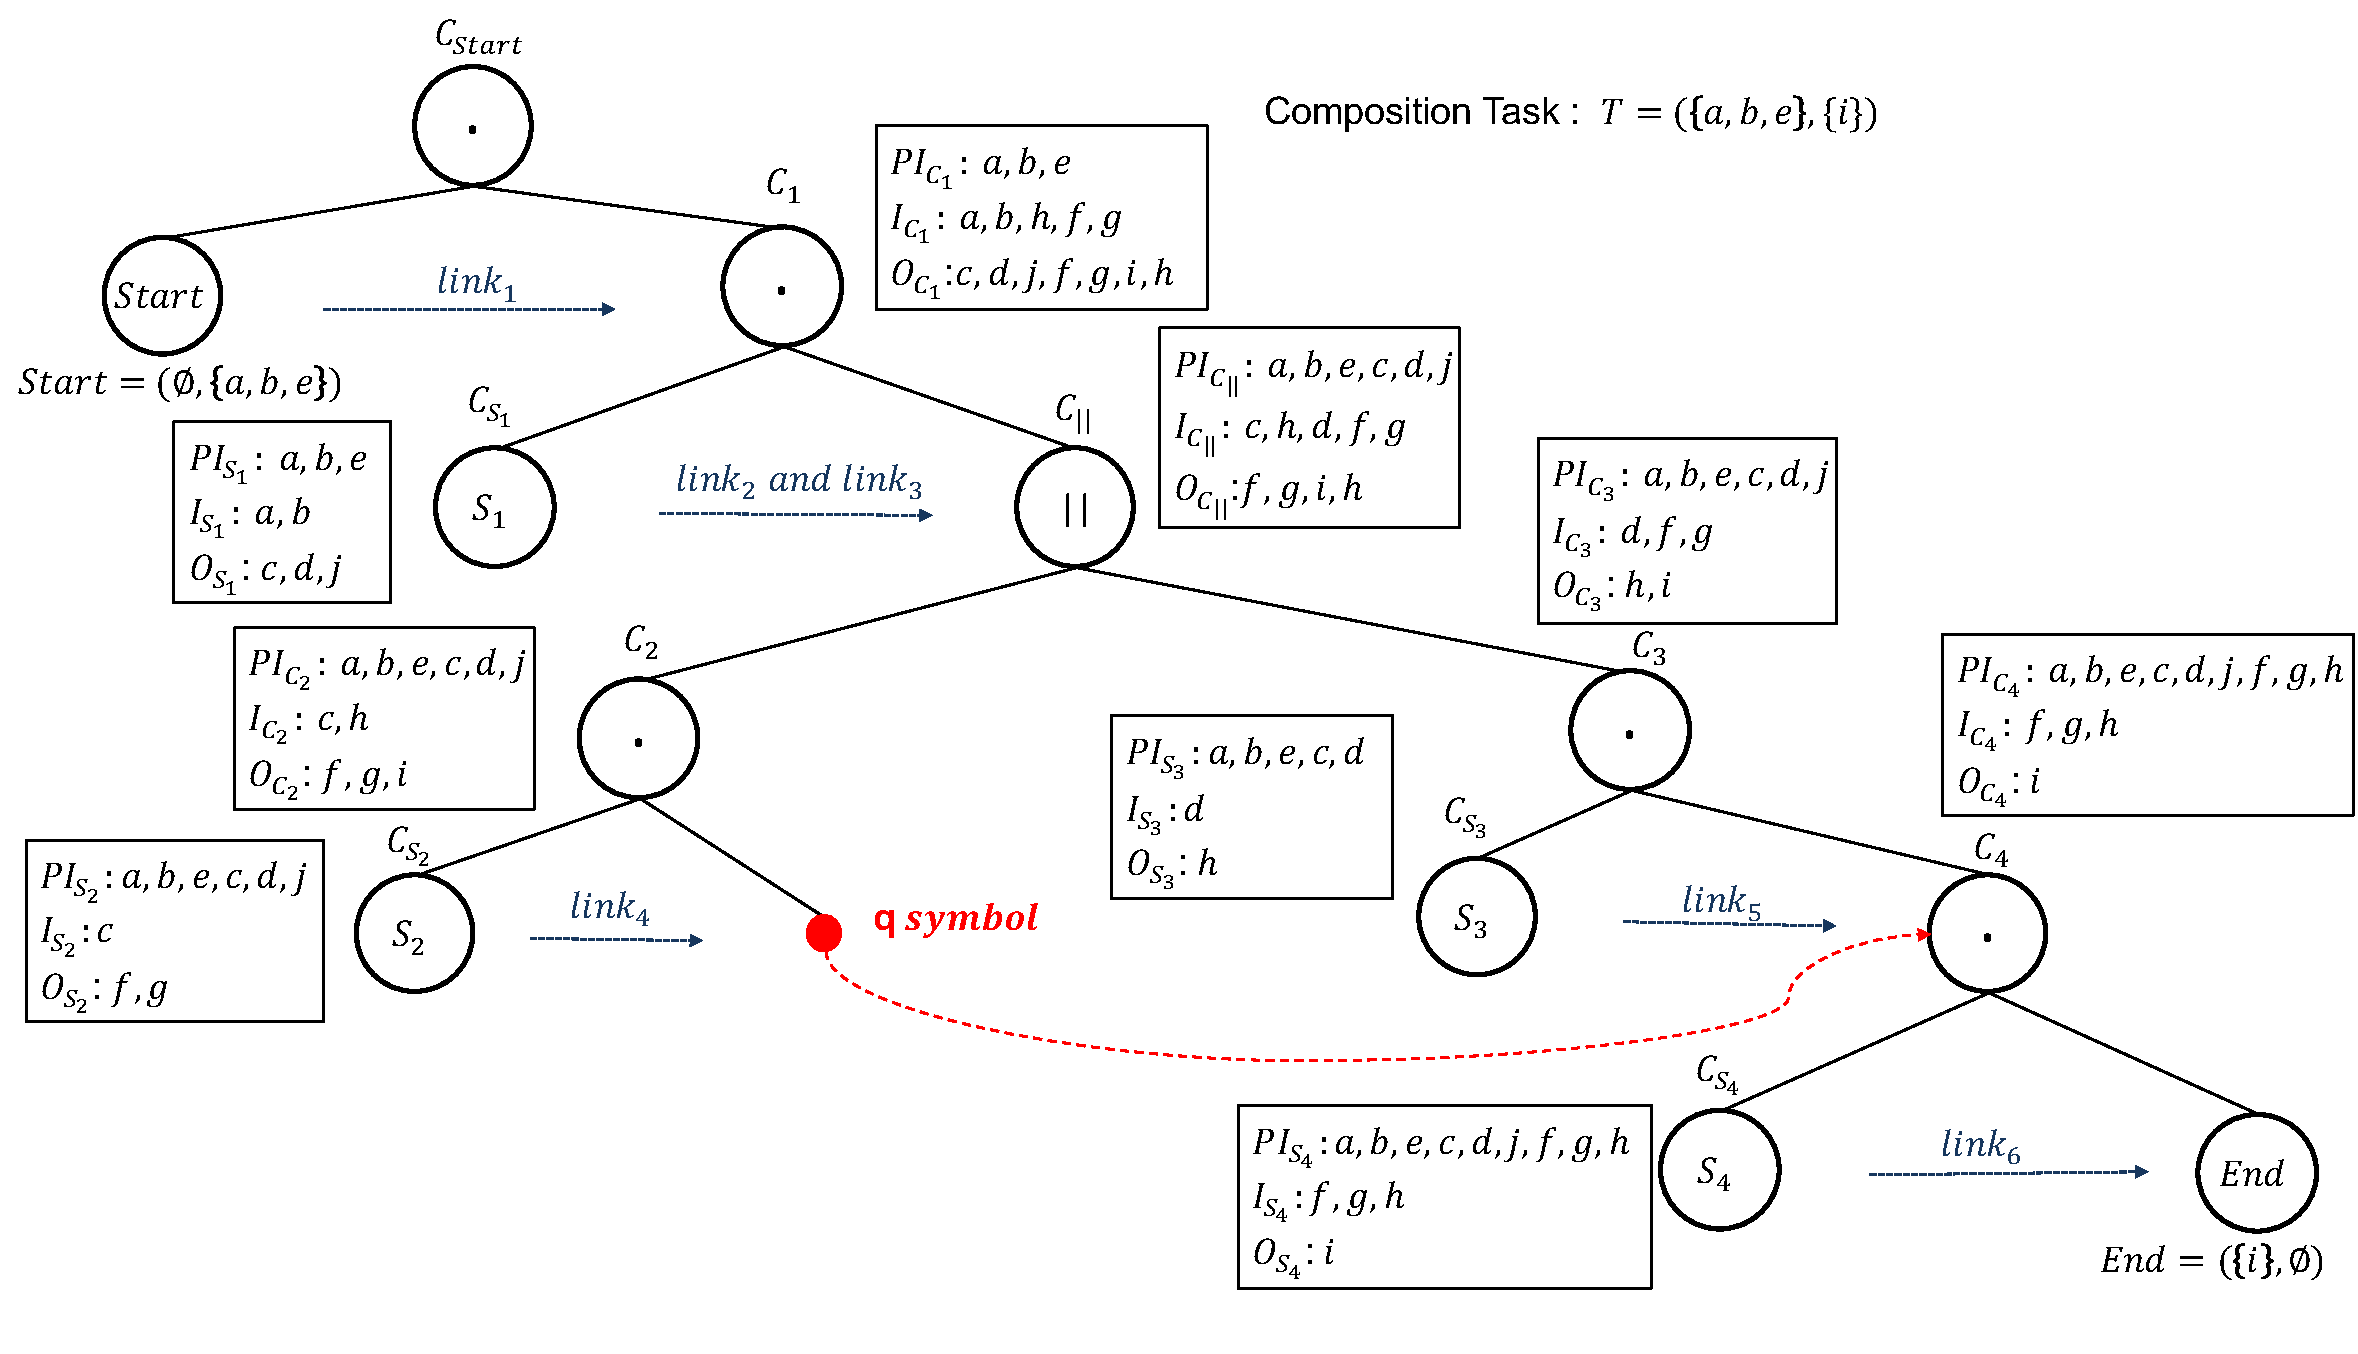
\includegraphics[width=1.0\textwidth]{Tree(p-symbol).pdf}}
 \caption{Example of a tree-like representation}
 \label{fig:ExampleOfRepresentation}
\end{figure}

%------------------- synthesis rules
Fig.~\ref{fig:ExampleOfRepresentation} shows for every atomic service $S$ its sets of (least required) inputs $\rin_S$ and outputs $\rout_S$. Moreover, the set of available inputs $\prin_S$ is shown which is just the union of the input sets of all (direct and indirect) predecessors of $S$ in the DAG.
%needs to be explained better
This can be easily generalized to composite service expressions. For a parallel composition $\cse=\parallel(\cse_1,\ldots,\cse_d)$ we define $\rin_\cse=\cup_{k=1}^d\rin_{\cse_k}$, and $\rout_\cse=\cup_{k=1}^d\rout_{\cse_k}$, and $\prin_\cse=\cup_{k=1}^d\prin_{\cse_k}$.
%we actually only need binary sequential compositions with a service in the first position
%not sure if this corresponds to what has been computed !!!
For a sequential composition $\cse=\bullet(S,\cse^\prime)$ we define $\rin_\cse=\rin_S\cup(\rin_{\cse^\prime}-\rout_S)$, and $\rout_\cse=\rout_S\cup\rout_{\cse^\prime}$, and $\prin_\cse=\prin_S$.
%more general we have:
%$\cse=\bullet(\cse_1,\ldots,\cse_d)$ we define $\rin_\cse=\rin_{\cse_1}\cup(\rin_{\cse_2}-\rout_{\cse_1})\cup\cdots\cup(\rin_{\cse_d}-\rout_{\cse_{d-1}})$ and $\rout_\cse=\rout_{\cse_1}\cup\cdots\cup \rout_{\cse_d}$, and $\prin_\cse=\prin_{\cse_1}\cup\cdots\cup \prin_{\cse_d}$. 

%------------------- new example
\begin{example}
%\cse here is actually \cse_{S_4}
Consider the sequential composition $\cse_4=\bullet(S_4, End)$ which is shown in the rightmost position in Fig.~\ref{fig:ExampleOfRepresentation}. We obtain $\rin_{\cse_4}=\{f, g, h\}$ which represents the (least required) inputs for this composition, and $\rout_{\cse_4}=\{i\}$ which represents the outputs produced by this composition, and $\prin_{\cse_4}=\{a, b, e, c, d, j, f, g, h\}$ which represents the union of the input sets of all (direct or indirect) predecessors of $S_4$ in the DAG (i.e., $S_1$, $S_2$ and $S_3$).
\end{example}

%\begin{example}
%Consider two atomic services $S_1$ with inputs $I_{S_1}=\{a,b\}$ and outputs $O_{S_1}=\{c,d\}$, and $S_2$ with inputs $I_{S_2}=\{c,d,e\}$ and outputs $O_{S_2}=\{f,g,h\}$. For their sequential composition $\cse=\bullet(S_1,S_2)$ we obtain $\rin_\cse=\{a,b,e\}$ which represents the least required inputs for this composition, $\rout_\cse=\{c,d,f,g,h\}$ which represents the outputs produced by this composition, and $\prin_\cse=\{a,b,e\}$ which represents the inputs that are provided by the predecessors of.
%this is not yet well described
%\end{example}

%\begin{figure}[h!tb]
%\centering
%%\fbox{\includegraphics[scale=.30]{synthesisRules.pdf}}
%\fbox{\includegraphics[width=.8\textwidth]{synthesisRules.pdf}}
% \caption{Example of representation and synthesis rules}
% \label{fig:ExampleOfSynthesisRules}
%\end{figure}

%Note that $\rin$, $\rout$ and $\prin$ can be computed recursively by tree traversal. For computing $\rin$ and $\rout$ we use pre-order depth-first traversal starting with the left-most leaf node of $Tree$, while for $\prin$ we use level-order breath-first traversal starting with the root node of $Tree$. 

%The representation used by our GP-based approach is a tree, $Tree = \{ V | \mathcal{R} \}$ with a set of nodes $V$ stored in a parent-child relationship $\mathcal{R}$ satisfying the following:
%\begin{enumerate}
%\item The node set $V = \{V_f,V_t\}$ consists of a set of functional nodes (internal nodes), $V_f = \{ \bullet, \parallel \}$, and a set of terminal nodes (leaf nodes), $V_t$=$\{Start, S_1, $ $S_2, \ldots, S_n, $ $End\}$. In $V_t$, $Start$ and $End$ are two special services defined as $Start = (\emptyset, I_T, \emptyset )$ and $End  = (O_T, \emptyset, \emptyset)$ that account for the input and output requirements given by the request $T$. 
 
%\item Each node $v \in V$ in $Tree$ is defined as a tuple $(I_{r}, O_{r}, I_{p}, QoS)$. The attributes $QoS$ are aforementioned in Sect. \ref{Problem Description}, while required inputs $I_r$, required outputs $O_r$ and provided inputs $I_p$ of $v$ are discussed here. $I_r$ is a set of inputs that is needed for executing the service composition represented in the subtree for which $v$ is the root node, and $O_r$ is obtained from the execution. $I_p$ of each $v \in V$ is a set of inputs available for $v$, which are obtained from two resources. One is from the task inputs $I_T$, and the other is from the outputs of $v$'s predecessor services in $Tree$, noted as $I_{pre}$.

%\item Some constrains are on $v \in V$ in $Tree$. The sequence node is always $\bullet(v_1 \in V_t, v_2 \in V)$ including two special cases for $Tree$'s $root$ and sequence constructs at the terminal level: $\bullet(Start, v_2 \in V_f)$ and $\bullet(v_1 \in V_t, End)$. The parallel node is always $\parallel(v_1\in V_f,..,v_n \in V_f)$, where $n\geq 2$.
%\end{enumerate}

Our representation supports composition constructs that are available in commonly used composition languages, such as BPEL4WS or OWL-S. Note that our representation is different from the most widely used tree-based representations in \cite{gupta2015optimization,da2016genetic,yu2013adaptive}. These differences are as follows.
\begin{enumerate}
\item $Start$ and $End$ are included in $\tree$, as they are related to measuring the semantic matchmaking qualities regarding $I_T$ and $O_T$.
\item $\rin_\cse$, $\rout_\cse$, $\prin_\cse$, $QoS_\cse$ are attributes, defined as a tuple $(\rin_\cse, \rout_\cse, \prin_\cse, QoS_\cse )$ for  any  $\cse_S$ in $\tree$. These attributes must be updated after population initialisation and genetic operations described in Sect. \ref{GP-Based Algorithm}.
\item $\tree$ preserves all the semantic matchmaking information, which can be easily used for computing robust casual links.
\end{enumerate}

%Based on and by extending the synthesis rules in \cite{fanjiang2014semantic}, we define a set of rules for computing $I_r$, $O_r$, $I_p$ of any $v \in V$ on $Tree$. The overall rules contain bottom-up and top-down methods to traverse $Tree$ recursively as follow: The bottom-up method for computing $I_r$, $O_r$ starts with the leftmost $v \in V_t$ in $Tree$ and continues to the right, then traverses the parent. On the other hand, the top-down method for calculating $I_p$ starts with the root of $Tree$, continues to traverse the children from the leftmost to the rightmost, then traverses the subtrees where each child is a root. During the traversal, $I_{r}$, $O_{r}$ and $I_{p}$ are updated in different ways according to each type of $v \in V_f$ as demonstrated in Fig. \ref{fig:ExampleOfSynthesisRules} $(b)$ and $(c)$. Note, for any $S(I_S, O_S) \in V_t$, $I_{r_{s}} = I_s$ and $O_{r_{s}} = O_s$.

%\begin{enumerate}
%\item If $v$ is $\bullet$, i.e.  $\bullet (S_1,S_2)$, when $S_1(\{a, b\}, \{c, d\}, QoS_1)$ and $S_2(\{c, d, e\}, \{f, g, h\}, $ $QoS_2)$, for $\bullet$, its $I_r = \{a, b, e \}$ is calculated by $I_{r_{1}} \cup (I_{r_{2}} \setminus  O_{r_{1}}) $, which presents the least required inputs for $\bullet$. Meanwhile, for $\bullet$, its $O_r = \{c, d, f, g, h \}$ is calculated by $O_{r_{1}} \cup O_{r_{2}}$, which presents all the output produced by $\bullet$. Suppose, for $\bullet$, its $I_{p}= \{a, b, e\}$ is inherited from the two resources ($I_T \cup I_{pre}$). For $S_1$, its $I_{p_{1}}= \{a, b, e\}$ as $I_{p}$ is passed to $S_1$. For $S_2$, its $I_{p_{2}} = \{a, b, e, c, d \}$ is calculated by $O_{r_{1}} \cup I_{p}$ as the both the inherited inputs produced $I_{p_{1}}$ and $O_{r_{1}}$ are included.

%\item If $v$ is $\parallel$, i.e. $\parallel(S_1,S_2)$, when $S_1(\{a, b\}, \{c, d\}, QoS_1)$ and $S_2(\{c, d, e\}, \{f,$ $ g, h\}, QoS_2)$, for $\parallel$, its $I_r = \{a, b, c, d, e \}$ is calculated by $ I_{r_{1}} \cup I_{r_{2}}$, which presents all the required inputs for $\parallel$. Meanwhile, for $\parallel$, its $O_r = \{c, d, f, g, h \}$ is calculated by $O_{r_{1}} \cup O_{r_{2}}$, which presents all the output produced by $\parallel$. Same as discussed above, for $\parallel$, its $I_{p} = \{a, b, e\}$ is inherited from the two resources ($I_T \cup I_{pre}$), For $S_1$ and $S_2$, $I_{p_{1}} = I_{p_{2}} = \{a, b, e\}$ as $I_{p}$ is passed to its children.
%\end{enumerate}


To compute semantic matchmaking quality, we need to retrieve all the robust causal links on $\tree$. This is performed by retrieving robust  causal links for every  sequential composition $\cse=\bullet(S,\cse^\prime)$. For example,  in Fig \ref{fig:ExampleOfRepresentation}, two robust causal links ($link_2: S_1 \rightarrow S_2$ and $link_3: S_1 \rightarrow S_3$ ) are retrieved from $\cse_1 = \bullet (S_1, \cse_{\parallel})$, because outputs $O_{S_1}=\{ c, d, j \}$ match inputs $I_{\cse_{\parallel}}=\{c, h, d, f, g\}$.


%\begin{algorithm}
% \setlength\hsize{0.9\linewidth}
% \SetKwInOut{Input}{Input}\SetKwInOut{Output}{Output}
% \SetKwFunction{evaluateSemanticLink}{evaluateSemanticLink}
% \SetKwProg{Procedure}{Procedure}{}{}
% \LinesNumbered
% \SetNlSty{}{}{:}
%  \Procedure{evaluateSemanticLink( ){}}{
% \Input{Tree $T$, IndexCache $cache$}
% \Output{Match type quality $MT$, Concept similarity $S$}
% \{ $ServNode \} \leftarrow  T.getAllServNode$\;
%     \ForEach{$ServNode$ in  \{ $ServNode$ \} }{
%      $NeighbourNode \leftarrow  ServNode.getNeighbourNode$\;
%    	 \ForEach{$O$ in $ServNode.outputs$ and $I$ in $NeighbourNode.requiredInputs$}{
%	  $mt_{P}, s_{P} \leftarrow$ query $cache(O,I)$\;
%	  $mt_{L} \leftarrow$ aggregation( $mt_{p}$ )\;
%	  $s_{L} \leftarrow$ aggregation( $s_{p}$ )\;
%	  \{$mt_{L}$ \} add $mt_{L}$\;
%	  \{$s_{L}$ \} add $s_{L}$\;
%        }
%       $MT \leftarrow$ aggregation( \{ $mt_{L}$\} )\;
%       $S \leftarrow$ aggregation( \{ $s_{L}$ \} )\;
%       }
% \KwRet $MT, S$\;
% }
% \caption{Evaluate semantic link in the tree.}
%\label{evaluateSemanticLink}
%\end{algorithm} 

%========================================================================================= Algorithm
\subsection{GP-Based Algorithm}\label{GP-Based Algorithm}

Now we present our GP-based approach for service composition, see Algorithm~\ref{GP-based algorithm}. To begin with the algorithm, we generate the initial population $P_0$, which is then evaluated using our comprehensive quality model. The iterative part of the algorithm comprises lines 3 to 7,  which will be repeated until the maximum number of generations is reached or the best solution is found. During each iteration, we use tournament selection to select individuals, on which crossover and/or mutation are performed to evolve the polulation. These steps correspond to the standard GP steps \cite{koza1992genetic} except for some particularities that will be discussed below.

%How do we know that we have found the best solution? In the algorithm below: where do we get max.fitness from?

\begin{algorithm}[h!tb]
 %\LinesNumbered
 \SetKwInOut{Input}{Input}\SetKwInOut{Output}{Output}
 \SetKwFunction{generateWeightedGraph}{generateWeightedGraph}
 \SetKwProg{Procedure}{Procedure}{}{}
 \SetNlSty{}{}{:}
 \Input{ $T$, $\mathcal{SR}$, $\mathcal{O}$}
 \Output{an optimal composition solution}
 Initialise population $P_0$ (using a 3-step method)\;
 Evaluate each individual in population $P_0$ (using our comprehensive quality model)\;
  \While {max.populations or max.fitness not yet met}{
     Select the fittest individuals for evolution\;
     Apply crossover and mutation to the selected individuals\;
%     Generate new individuals\;
     Evaluate each new individual\;
     Replace the individuals with the smallest fitness in the population by the new individuals\;
  }
 Find the individual with the highest fitness in the final population\;
\caption{GP-based algorithm for service composition.}
\label{GP-based algorithm}
\end{algorithm} 

\textbf{Population initialisation.}
The initial population is created by generating a set of service compositions in form of DAGs, and then transforming them into their tree-like representations (\emph{the individuals}). The initialisation is performed as follows: 

%Should we explain when a DAG is valid service composition solution?
\textsc{Step 1}. Greedy search is performed to randomly generate a set of DAGs, each representing a (valid) service composition for the given composition task $T$. For this, a simple forward graph building algorithm is applied starting with the node $Start$ and the inputs $I_T$ of the composition task $T$. Details of this algorithm can be found in \cite{ma2015hybrid}. An example of a generated DAG is shown in Fig.~\ref{fig:DAG} with seven robust casual links marked on.

\textsc{Step 2}. The DAGs can be simplified by removing some redundant edges and service nodes. 
%We formalise the criteria for identifying such edges: The outgoing edges from an atomic service $S$ to its direct successors are considered for removal if the direct successors overlap with their successors. This criterion is checked from $Start$ to $End$. 
While this step is not compulsory, it can help to notably reduce the size of the DAG and, consequently, the corresponding tree-like representation. 

\textsc{Step 3}. 
%For each DAG we initialize an auxiliary data structure to record the available inputs for every service node in the DAG. 
We transform each DAG into its tree-like representation using an algorithm modified from \cite{da2016genetic} to satisfy the particular requirements of our proposed approach. For example, Fig.~\ref{fig:ExampleOfRepresentation} shows an example of a tree-like individual corresponding to the DAG shown in Fig.~\ref{fig:DAG}.

%\begin{example}
%Fig.~\ref{DAG} illustrates the generation and simplification of a DAG.  The  corresponding tree shown in Fig.~\ref{fig:ExampleOfRepresentation} is transferred from this DAG. In the initial DAG, service $S_4$ requires the inputs produced by $S_1$, $S_2$ and $S_3$. However, $S_4$ can not be invoked until both $S_2$ and $S_3$ are executed. Therefore, we can simplify the DAG by removing the edge between $S_1$ and $S_4$ (noted as $link_7$) without impacting the execution of a service composition. To transform the DAG into a tree, we traverse the DAG from $Start$ to $End$ with a cursor to mark the current position while creating a node in the tree according to the cursor's position and the number of outgoing edges. In addition, seven robust casual links marked in this DAG could be retrieved from transferred tree in Fig.~\ref{fig:ExampleOfRepresentation} .
%\end{example}

\begin{figure}[htb]
\centering
%\fbox{\includegraphics[scale=.30]{transformationExample.pdf}}
\fbox{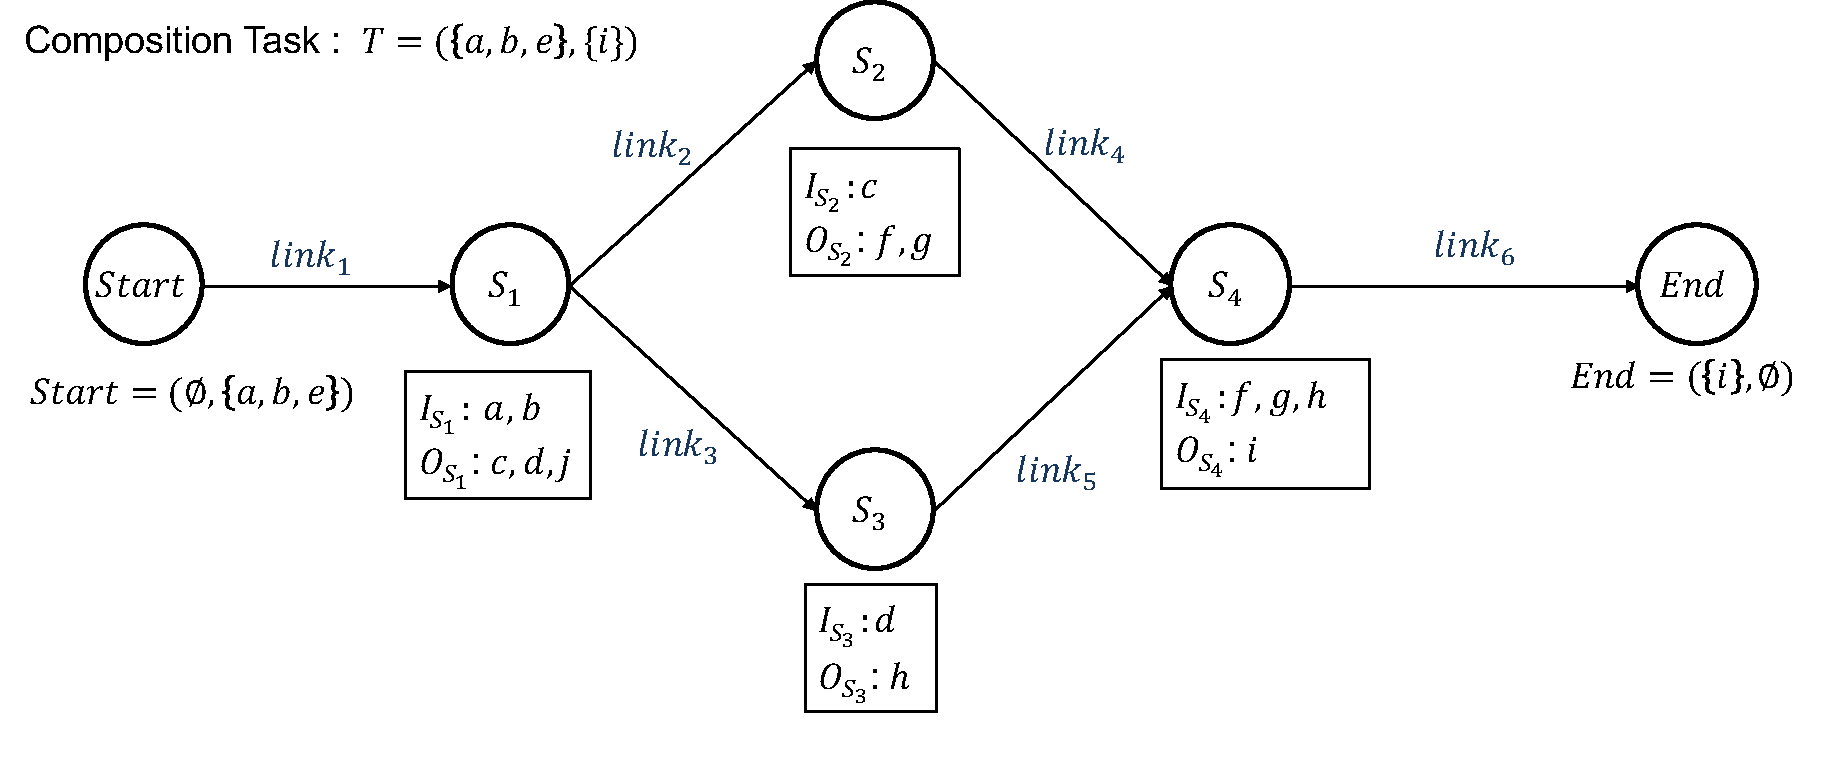
\includegraphics[width=.7\textwidth]{DAG(p-symbol).pdf}}
 \caption{Example of a weighted DAG used for transferring it into tree-like representation}
 \label{fig:DAG}
\end{figure}


%\begin{figure}[htb]
%\centering
%%\fbox{\includegraphics[scale=.30]{transformationExample.pdf}}
%\fbox{\includegraphics[width=.8\textwidth]{transformationExample.pdf}}
% \caption{Example for the transformation of the DAG for a service composition into its tree-like representation}
% \label{transformationExample}
%\end{figure}

%This section still needs to be modified. I can describe crossover and mutation similar to the GraphEvol approach (though these are a bit more restrictive than the crossover and mutation considered so far in this paper). Or I can describe it a bit more general or even leave it somewhat open.
%Later we need an example. The solution of Dataset 3 is a possible example, but a bit small. I would like to see the solution of Dataset 4 before I can say what a good example would be.
\textbf{Crossover and Mutation.} 
During the evolutionary process, the correctness of the representation is maintained by crossover and mutation. 

A crossover operation exchanges a subtree of a selected individual (its attributes noted as $\cse_1 (\rin_{\cse_1}, \rout_{\cse_1}, \prin_{\cse_1}, QoS_{\cse_1})$) with the subtree of another selected individual (its attributes noted as $\cse_2 (\rin_{\cse_2}, \rout_{\cse_2}, \prin_{\cse_2}, QoS_{\cse_2})$) 
if they represent the same functionality (i.e. $\rin_{\cse_1} = \rin_{\cse_2}$ and $\rout_{\cse_1} = \rout_{\cse_2}$). That is, at the root nodes of both subtrees, we have identical inputs and identical outputs. A crossover operation is performed in two cases: crossover on two functional nodes or on two terminal nodes. We never exchange a functional node with an terminal node, since the two associated subtrees cannot be equivalent in this case. For example, $End$ must appear in the subtree associated with any functional node, but not for any selected terminal node (atomic services). 
%\begin{figure}[h]
%\centering
%\fbox{\includegraphics[scale=.26]{crossoverExample.pdf}}
% \caption{Example of a crossover}
% \label{crossoverExample}
%\end{figure}

A mutation operation replaces a subtree of the selected individual (its attributes noted as $\cse_1 (\rin_{\cse_1}, \rout_{\cse_1}, \prin_{\cse_1}, QoS_{\cse_1})$) with a newly generated subtree satisfying the least required functionality. To do this, a subtree $\cse_1$ must be selected from the selected individual, and a new composition task $T=(\{\prin_{\cse_1}\},\{\rout_{\cse_1} \cap O_T\})$ or $T'=(\{\prin_{\cse_1}\},\{\rout_{\cse_1}\})$ is used to generate a tree in the same way as the 3-step method performed during the population initialisation. We utilise the available inputs and least required outputs for mutation, because it potentially bring more possibilities in generating more varieties of subtrees. The mutation is performed in two cases: mutation on a functional node with $T$ or on a service node with $T'$, two examples shown in Fig \ref{mutationExample} $(a)$ and $(b)$. In Fig \ref{mutationExample} $(a)$, a functional node $\cse_{\parallel}$ is selected for mutation, the whole subtree is replaced with the generated subtree excluding its head (i.e., $Start$ and its parent node $\bullet$). In Fig \ref{mutationExample} $(b)$, a atomic service $S_1$ is selected for mutation, the branch of the selected node (i.e., $S_1$ and its parent node $\bullet$) is replaced with the generated subtree excluding both its head (i.e., $Start$ and its parent node $\bullet$) and its tail (i.e., $End$).

\begin{figure}[h!tb]
\centering
%\fbox{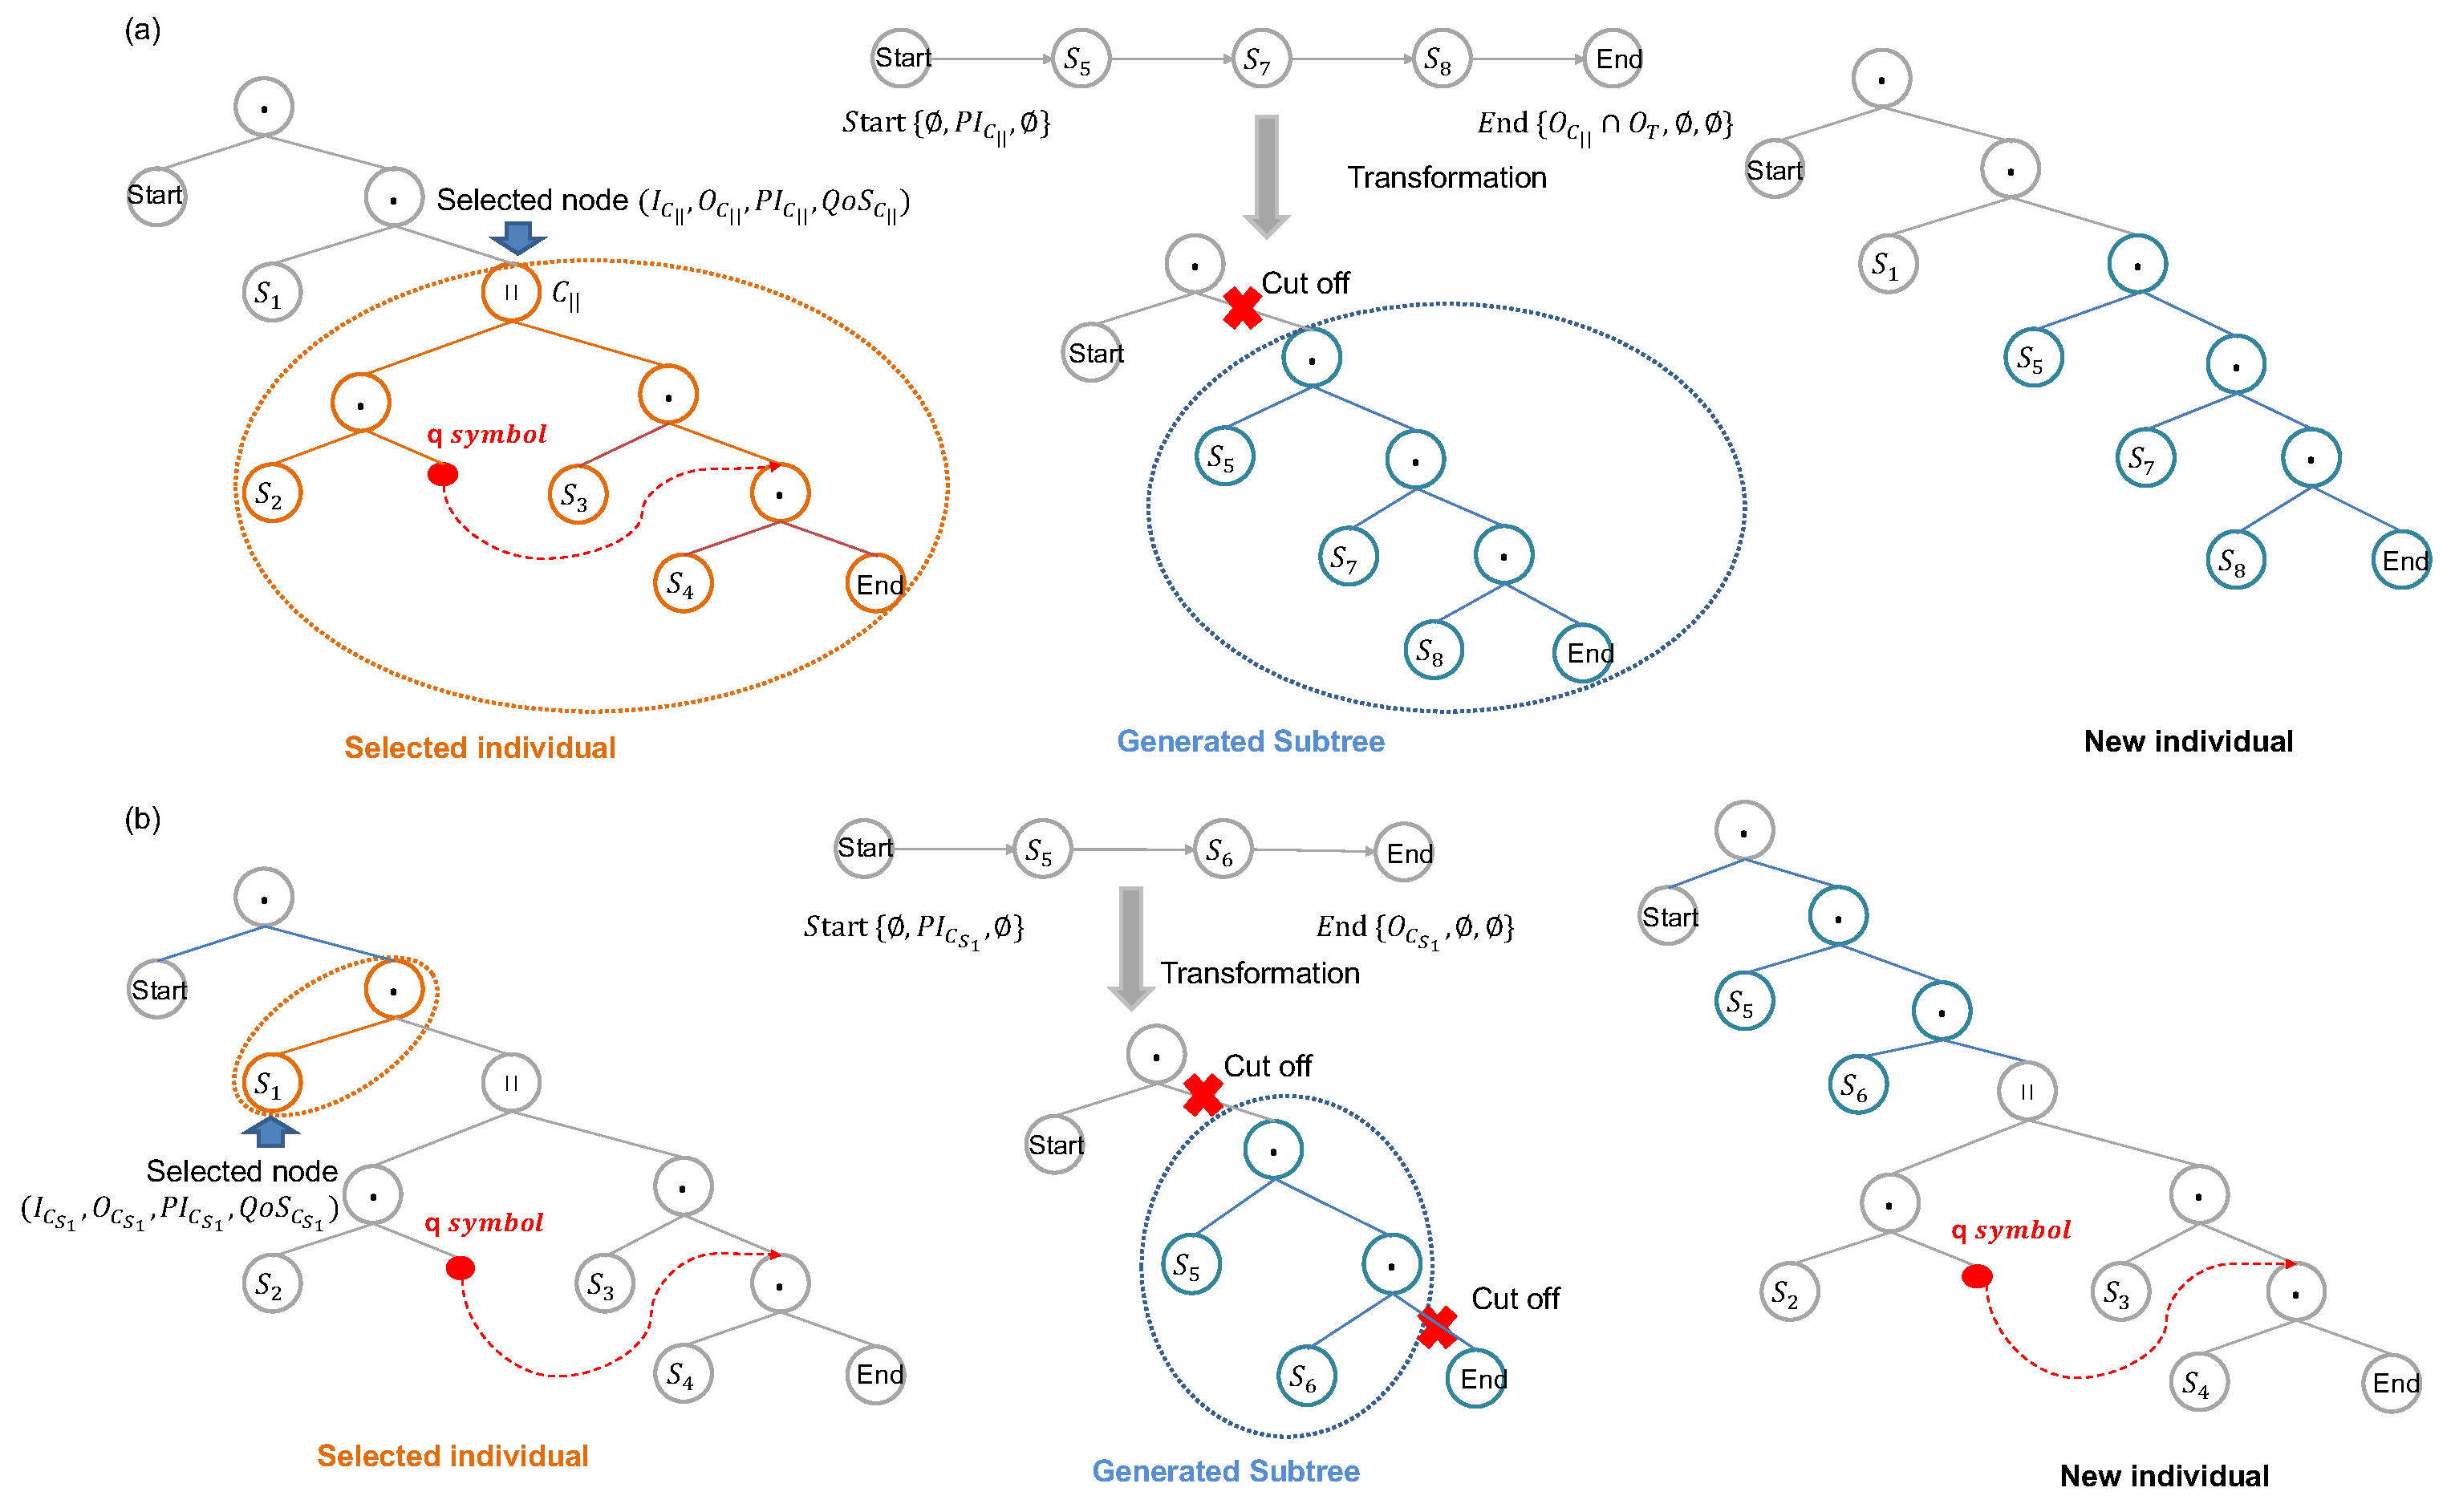
\includegraphics[scale=.23]{mutationExample.pdf}}
\fbox{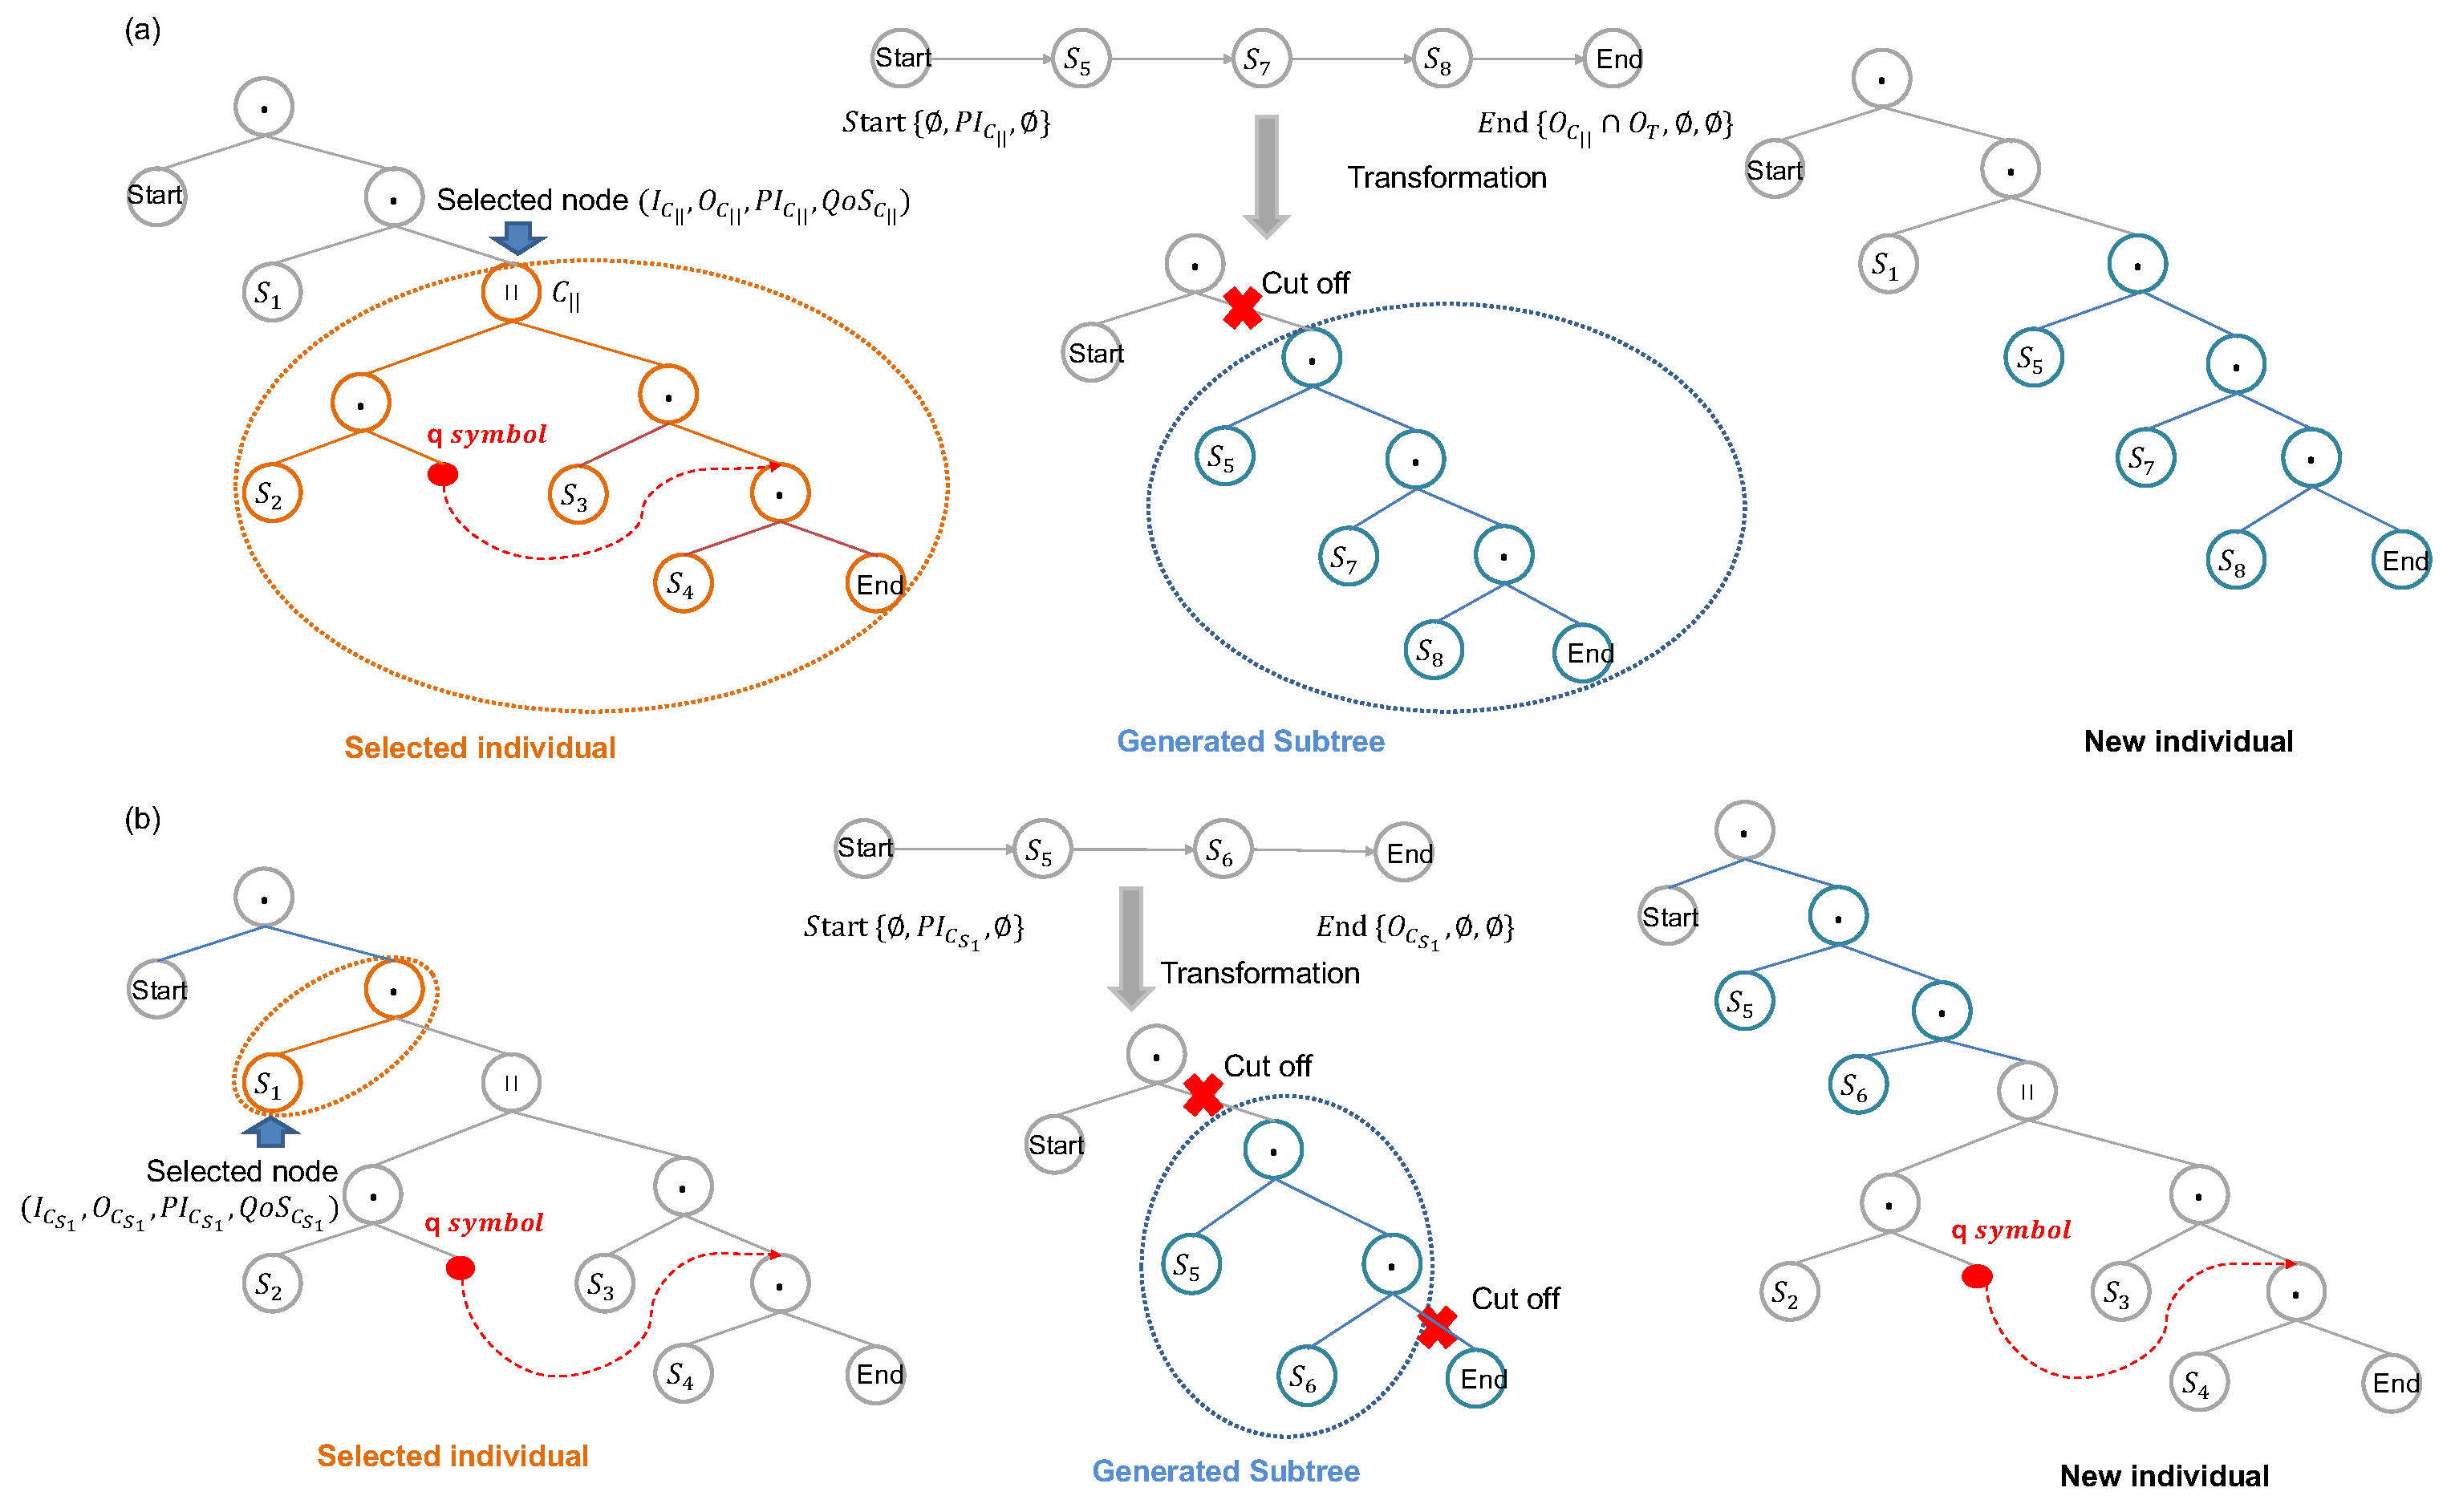
\includegraphics[width=\textwidth]{mutationExample.pdf}}
 \caption{Examples of two mutations on terminal and functional nodes}
 \label{mutationExample}
\end{figure}

Note: The set of available nodes considered for crossover  and mutation do not include $Start$ and $End$, and their parent nodes, because these nodes remain the same for all individuals.  In addition, the nodes selected for crossover and mutation must not break the functionality of $q$ symbols. For example, in Fig. \ref{fig:ExampleOfRepresentation}, both sequential composition $\cse_2$ and $\cse_3 $ are not considered for crossover and mutation as they break the edge of $q$ symbol, but the parallel composition $\cse_{\parallel}$ can be considered for genetic operations, as it may bring a new fully functional $q$ symbol or a subtree without $q$ symbol involved. The pointed subtree $\cse_4$ could also be selected for genetic operations. 
%=================================================================================================== Experiments
\section{Experiment Study for GP-based Approach}\label{experiment_study}

We have conducted experiments to evaluate our proposed approach. 
For our experiments we have used the benchmark datasets originating from OWLS-TC \cite{kuster2008opossum} , which have been extended with real-world QoS attributes and five composition tasks \cite{ma2015hybrid}. To explore the effectiveness and efficiency of our proposed GP-based approach, we compare it against one recent GP-based approach \cite{ma2015hybrid}. For that we have extended the later approach by our proposed comprehensive quality model, so that semantic matchmaking quality can be computed based on the parent-child relationship in the underlying tree representations. 

%Describe the computer environment that you have used for your experiments!

To assure a fair comparison we have used exactly the same parameter settings as in \cite{ma2015hybrid}. In particular, the GP population size has been set to 200, the number of generations to 30, the reproduction rate to 0.1, the crossover rate to 0.8, and the mutation rate to 0.1. We have run every experiment with 30 independent repetitions. Without considering any users' true service composition preferences, the weights in fitness function in Eq. (\ref{eq_fitness}) have been are configured simply to balance semantic matchmaking quality and QoS. Particularly, $w_{1}$ and $w_{2}$ are both set to 0.25, while $w_{3}$, $w_{4}$, $w_{5}$, and $w_{6}$ are all set to 0.125. The parameter $p$ of $type_{link}$ is set to 0.75 ($plugin$ match) in accordance with the recommendation in \cite{lecue2009optimizing}. 

%Why is it fair to use the same parameter settings as in \cite{ma2015hybrid}? Wouldn't it be fair to choose parameter settings that we like and then run experiments with both approaches using the same parameter settings?

Our experiments indicate that our method can work consistently well under valid weight settings and parameter $p$ to be decided by users' preferences in practice.

%========================================================================================= Comparison
\subsection{Comparison against a previous GP-based approach}\label{comparisonTest2}

Table~\ref{meanFitness_GP} shows the fitness values obtained by the two GP-based approaches. To compare the results, an independent-samples T-test over 30 runs has been conducted. The results show that our GP-based approach outperforms the previous GP-based approach \cite{ma2015hybrid} in finding more optimized composition solutions for Tasks 3 and 4. (Note: the P-values are lower than 0.0001). For Tasks 1, 2 and 5, both approaches achieve the same fitness. Therefore, the overall effectiveness of our proposed approach is considered to be better. 

%Why have we conducted a independent-samples T-test rather than a Wilcoxon test?
%We should explain better what we want to emphasize by saying "note: the P-values are lower than 0.0001"
\begin{table}[h!tb]
\footnotesize
\centering
\caption{Mean fitness values for our approach in comparison to \cite{ma2015hybrid}\\ (Note: the higher the fitness the better)}
\label{meanFitness_GP}
\begin{tabular}{l|l|l}
\hline
\multicolumn{1}{c|}{Task} & Our GP-based approach                  & Ma et al. approach \cite{ma2015hybrid}  \\ \hline
OWL-S TC1                     & 0.923793 $\pm$ 0.000000                & 0.923793 $\pm$ 0.000000                   \\ \hline
OWL-S TC2                     & 0.933026 $\pm$ 0.000000                & 0.933026 $\pm$ 0.000000                   \\ \hline
OWL-S TC3                     & 0.870251 $\pm$ 0.000000 $\uparrow$     & 0.832306 $\pm$ 0.008241                   \\ \hline
OWL-S TC4                     & 0.798137 $\pm$ 0.007412 $\uparrow$     & 0.760146 $\pm$ 0.005044                   \\ \hline
OWL-S TC5                     & 0.832998 $\pm$ 0.000000                & 0.832998 $\pm$ 0.000000                   \\ \hline
\end{tabular}
\end{table}

Table~\ref{meanTime} shows the execution times observed for the two GP-based approaches. Again an independent-samples T-test over 30 runs has been conducted. For Tasks 1 and 2 both approaches need about the same time, while for Tasks 3,4, and 5 our approach needs slightly more time. (Note: the P-values are lower than 0.0001). However, even in the worst case it exceeds \cite{ma2015hybrid} by no more than 1 second, which is acceptable for most real-word scenarios. Hence, in terms of efficiency our approach is comparable to \cite{ma2015hybrid}.
\begin{table}[h!tb]
\footnotesize
\centering
\caption{Mean execution time (in ms) for our approach in comparison to \cite{ma2015hybrid}\\ (Note: the shorter the time the better)}
\label{meanTime}
\begin{tabular}{l|l|l}
\hline
\multicolumn{1}{c|}{Task} & Our GP-based approach            & Ma et al. approach \cite{ma2015hybrid}     \\ \hline
OWL-S TC1                     & 7396.366667 $\pm$  772.408168    &  7310.866667  $\pm$952.701775                       \\ \hline
OWL-S TC2                     & 2956.133333  $\pm$ 761.350965    &  3036.966667 $\pm$ 777.121101                       \\ \hline
OWL-S TC3                     & 1057.266667  $\pm$ 174.405183    &  763.800000 $\pm$ 221.241232  $\downarrow$          \\ \hline
OWL-S TC4                     & 4479.466667  $\pm$ 519.767172    &  3068.800000 $\pm$ 472.013106  $\downarrow$        \\ \hline
OWL-S TC5                     & 6276.533333  $\pm$ 1075.102328   &  5030.200000 $\pm$ 991.863812 $\downarrow$         \\ \hline
\end{tabular}
\end{table}

The experiments confirm that there is a trade-off between fitness and execution time in GP-based service composition. It can be argued that our proposed approach achieves a better balance as the computed solutions observe a significantly higher fitness while there is a moderate increase in execution time compared to \cite{ma2015hybrid}. 

%========================================================================================= Discussion
\subsection{Further Discussion}
For Tasks 3 and 4, the optimized composition solutions obtained by the two approaches are shown in Fig.~\ref{example1and2}(a) and Fig.~\ref{example1and2}(b), respectively. The functional and nonfunctional descriptions of all services involved in these solutions are listed in Fig.~\ref{example1and2}(c). 

%For Datasets 3 and 5, the optimized composition solutions obtained by the two approaches are shown in Fig.~\ref{example1and2}(a) and Fig.~\ref{example1and2}(b), respectively. The functional descriptions of all services involved in these solutions are listed in Fig.~\ref{example1and2}(c). For Dataset 5 the composition task is $T=( \{ duration, city, country \}, \{ weatherseason, map, hotel\})$. The optimized composition solutions obtained by the two approaches are identical, even though different representations have been used during GP.  

%change "Task" to "Dataset" in the figure,
% there is only one dataset with 5 different tasks
%Should we move the composition task into the figure so that readers don't need to look for it in the text?

\begin{figure}[h!tb]
\centering
%\fbox{\includegraphics[scale=.30]{example1and2.pdf}}
\fbox{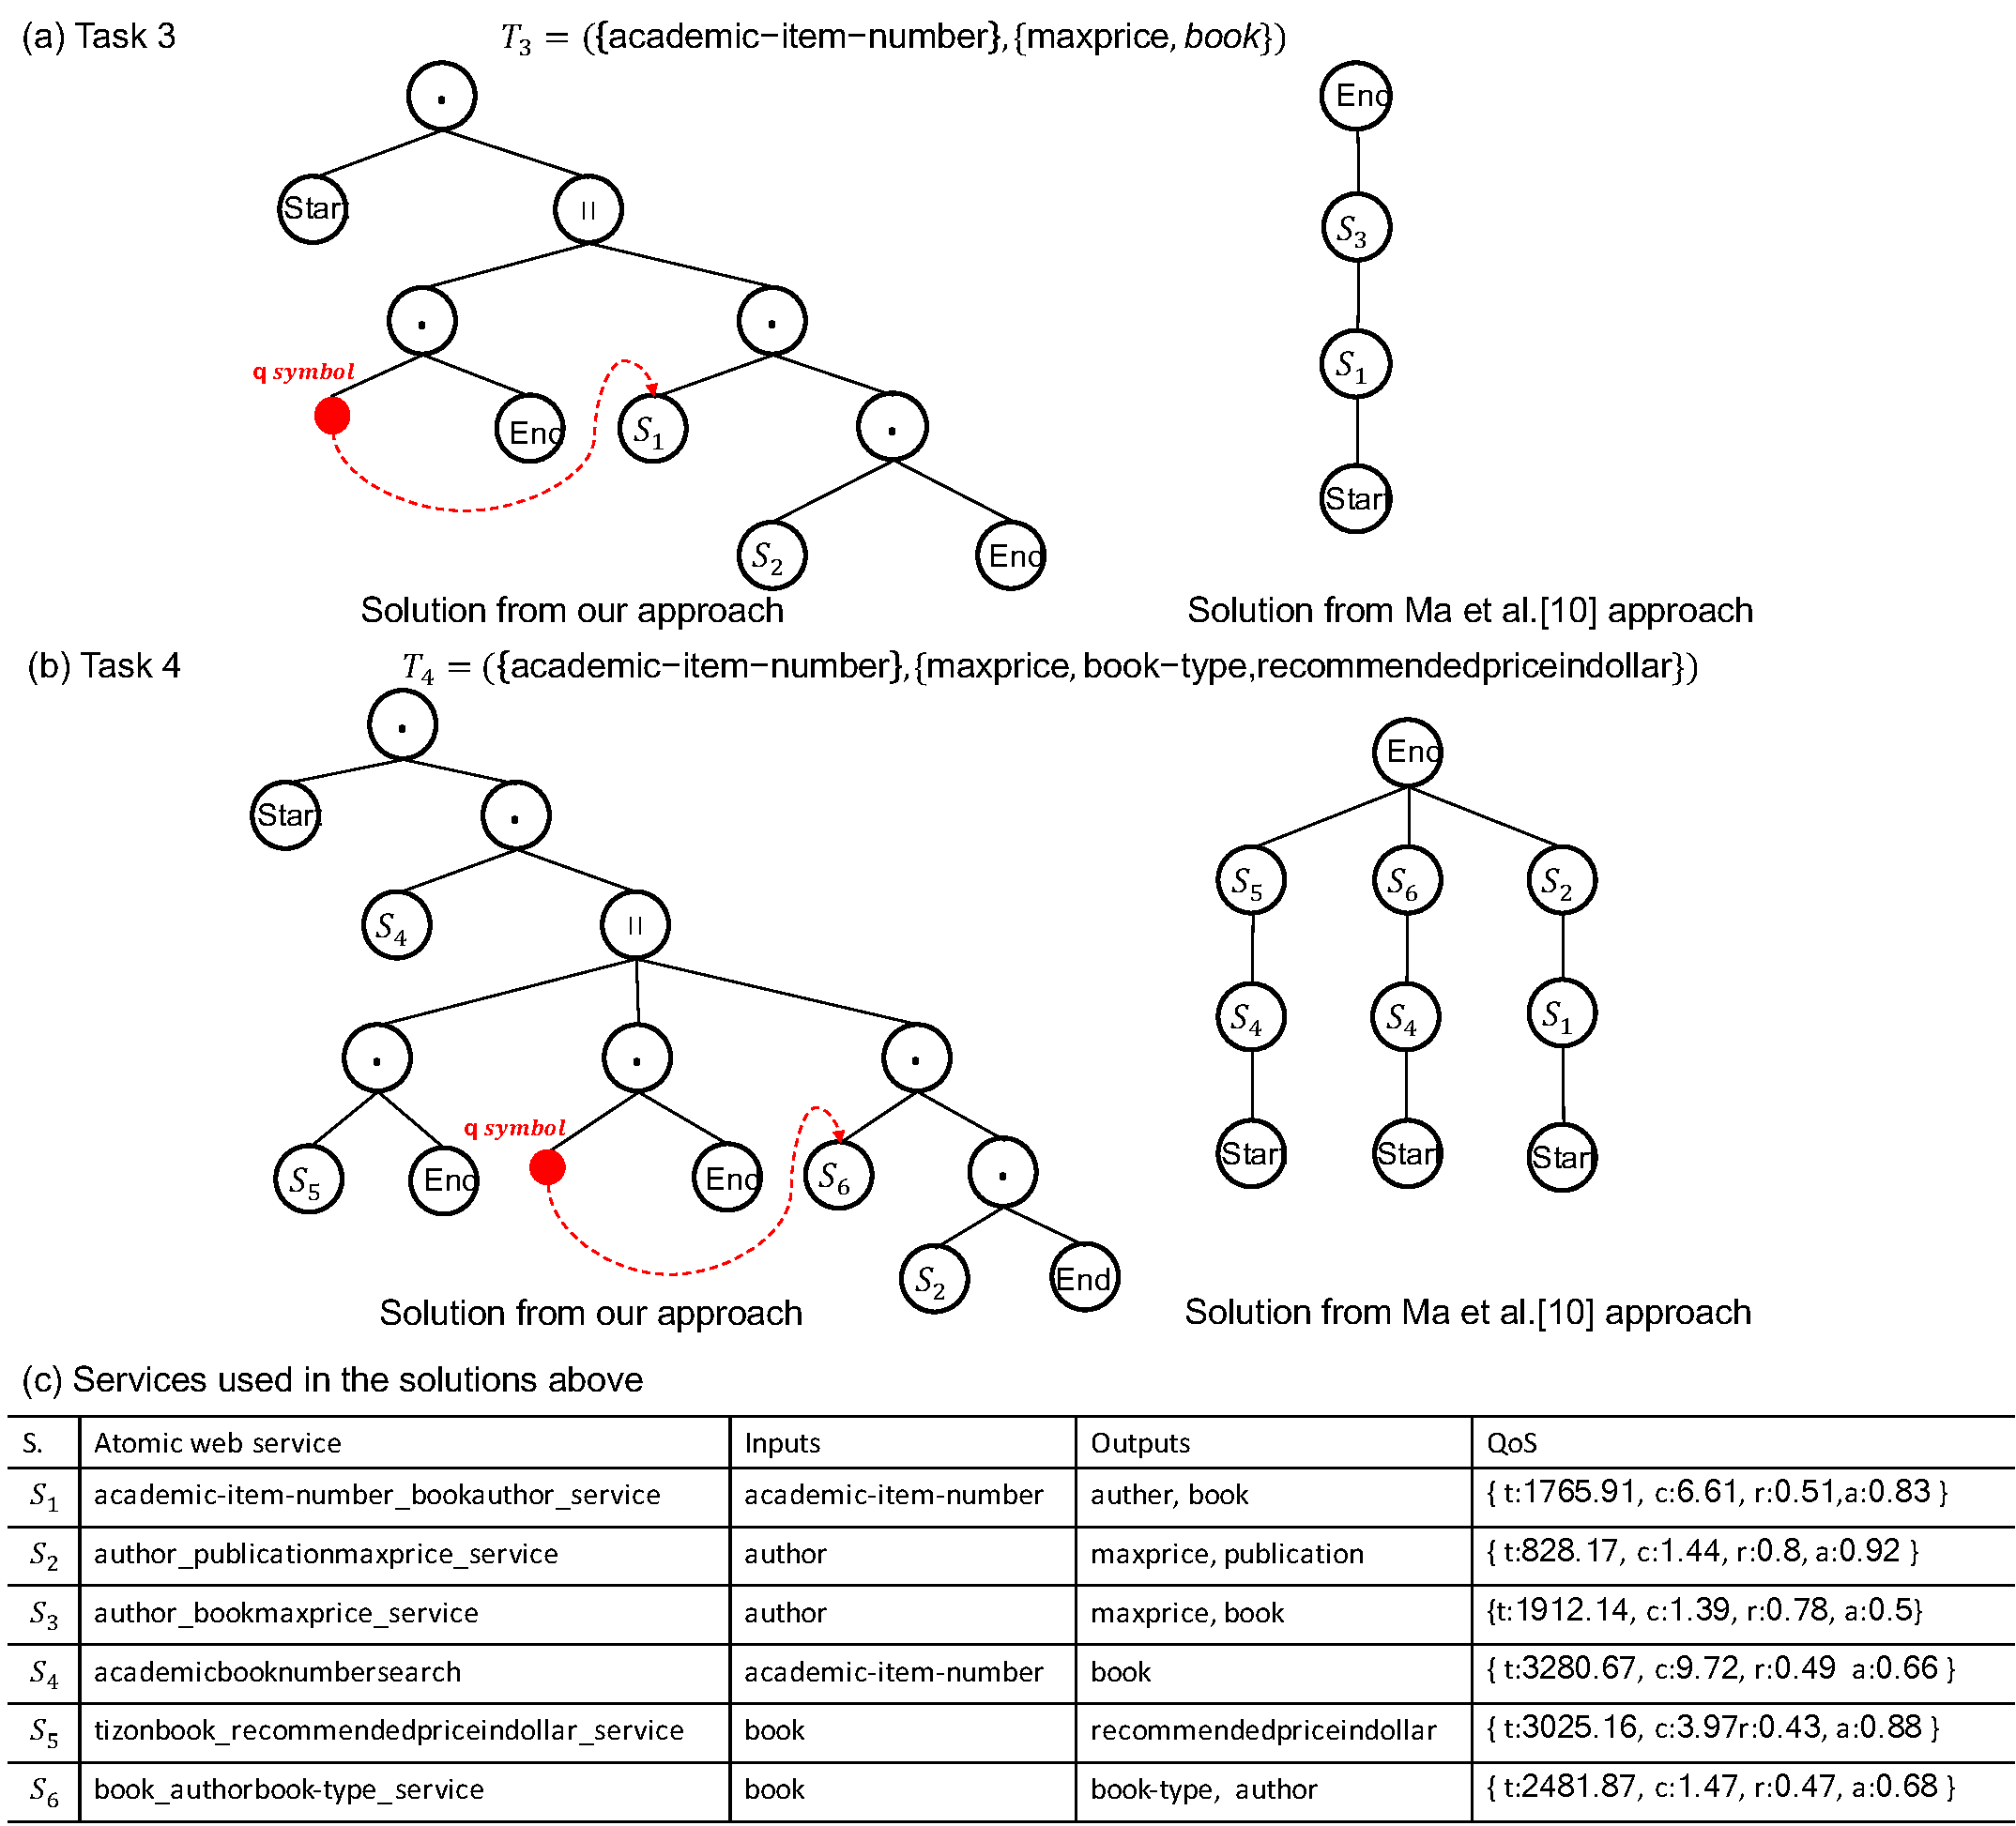
\includegraphics[width=.9\textwidth]{experimentExample(p-symbol).pdf}}
 \caption{Example of best solutions using the two GP-based approaches}
 \label{example1and2}
\end{figure}
\noindent For Task 3 the composition task is $T_3=(\{academic$-$item$-$number\},\{ book, maxprice\})$. The best composition solutions obtained by the two approaches are different, see Fig.~\ref{example1and2}. Both solutions have the same semantic matchmaking quality as the matchmaking type of all links is $exact$ match. However, both solutions differ in their QoS. This is due to the different services that are involved: $S_2$ versus $S_3$. The QoS of $S_2$ is much better that of $S_3$. Consequently, the best composition solution obtained by our approach has higher fitness according to our quality model.  It is interesting to observe that the best composition solution obtained by our approach for Task 3 can be evolved from the best composition solution in  \cite{ma2015hybrid} just by a single mutation on $S_3$ using available inputs.


For Task 4 the composition task is $T_4=(\{academic$-$item$-$number\},\{ maxprice, book-type,recommendedpriceindollar\})$. The best solutions obtained by the two approaches are also different, see Fig.~\ref{example1and2}. Note that solution generated by our approach is composed of four atomic services ($S_4$, $S_5$, $S_6$ and $S_2$) while the solution generated by approach \cite{ma2015hybrid} is composed of  five atomic services ($S_4$, $S_5$, $S_6$, $S_1$ and $S_2$). Both solutions have the same semantic matchmaking quality as the matchmaking type of all links is $exact$ match. However, the overall QoS of our approach is better. This is due to the additional $S_1$ in their approach, which has a significant negative impact on QoS.

We observe from above examples that our approach is able to produce better solutions because our proposed representation keeps available inputs and least required outputs of each node on the tree which unlocks more opportunities for 
mutation and crossover rather than restricting them to the previously used inputs and outputs only.

%\begin{figure}[h!tb]
%\centering
%\fbox{\includegraphics[scale=.30]{example1and2.pdf}}
%\fbox{\includegraphics[width=.9\textwidth]{example1and2.pdf}}
% \caption{Example of best solutions using the two GP-based approaches}
% \label{example1and2}
%\end{figure}

%It may due to the structure of the introduced representation that brings more possibilities of different combined functionality via functional nodes and more flexible mutation operator that utilises available inputs to generate more varieties of subtrees.

%How about the best solutions obtained with both approaches for Dataset 4? Can we look at them?
%=================================================================================================== Conclusion
\section{Summary for our GP-based Approach}\label{summary2}

In this work, we introduces a novel GP-based approach to comprehensive quality-aware semantic web service composition. In particular, a tree-like representation is proposed to direct cope with the evaluation of semantic matchmaking quality. Meanwhile, crossover and mutation methods are proposed to maintain the correctness of individuals. The experiment  shows that our proposed approach could effectively produce better solutions in both semantic matchmaking quality and QoS than the existing approach.

\section{Conclusion}\label{summary2}
In the preliminary work, we propose and formalize a novel and effective comprehensive quality model for simultaneously optimize QoS and quality of semantic matchmaking. Apart from that, two novel and effective EC-based methods are proposed for comprehensive quality-aware semantic web service composition. In particular, indirect and direct representations are designed for studying their effectiveness and efficiency along with newly developed evolutionary operators. Overall experimental studies show both two methods reach good performances comparing to existing works. We also find that our PSO-based approach utilizing an indirect representation outperforms our GP-based approach utilizing a direct representation for finding more effective solutions. These findings motivate us to work on a more effective indirect presentation along with PSO-based memetic method.
%=================================================================================================== Bibliography
%The bibliography can be improved. Remove unnecessary bibliographic information from some of the items. Make sure that QoS is not shown as qos.
